\documentclass[preprint,12pt]{elsarticle}

\usepackage{amsmath,amssymb,amsthm}
\usepackage{graphicx}
\usepackage{booktabs}
\usepackage{multirow}
\usepackage{adjustbox}
\usepackage{xcolor}
\usepackage{tikz}
\usetikzlibrary{positioning,arrows.meta}
\usepackage[hidelinks]{hyperref}
\usepackage{lineno}

\newtheorem{proposition}{Proposition}
\makeatletter\let\inputtable\@@input\makeatother
\graphicspath{{figures/}}

\journal{Engineering Structures}

\begin{document}

\begin{frontmatter}

\title{A mechanics-constrained surrogate modelling framework for rapid structural response prediction with adaptive finite element data generation}

\author[1]{Karthik Research\corref{cor1}}
\ead{karthikresearchworks@gmail.com}
\cortext[cor1]{Corresponding author. Author names and affiliations are placeholders to be completed by the authors before submission.}
\affiliation[1]{organization={Affiliation to be completed},
            country={Country}}

\begin{abstract}
Data-driven surrogates of finite element (FE) models can accelerate repeated structural assessment, but their member forces usually violate equilibrium and they give no indication of when they should not be trusted. This paper develops equilibrium-projected graph neural network surrogates for the first-order linear analysis of planar moment frames, with every analysis run in the open-source PyNite library and verified against an independent stiffness solver, OpenSeesPy and closed-form solutions. A graph network ensemble predicts all nodal displacements and member forces in a dimensionless, load-case-separated form, so that superposition, homogeneity in the loads, the $1/E$ scaling of displacements and the boundary conditions hold exactly. A projection in a variance-weighted metric maps the predicted forces to the nearest field in static equilibrium. Two indicators are used for two different decisions: at deployment, a domain check on geometry and load-pattern descriptors followed by a split-conformal bound on the ensemble spread decides which frames are referred back to the FE solver; during training, the equilibrium residual of the raw prediction decides which frames receive new FE analyses. On 7{,}500 PyNite analyses and five independent training runs, the median end-moment error was $2.37\pm0.03\%$ on in-distribution frames and $1.99\pm0.08\%$ on design-driven frames, four to nine times lower than five tabular baselines given the same features; a StructGNN-style network reached similar accuracy, and displacement-only networks with force recovery were much less accurate. On unseen geometries and load patterns the median moment errors rose to 7.5\% and 8.7\%, with 95th percentiles above 20\%. The projection reduced nodal out-of-balance forces from 4--16\% to below $10^{-12}$ and the axial-force errors by factors of 2--5, but changed the moment errors only modestly. With thresholds fixed on validation data, the referral rule accepted 98\% of in-distribution frames with 1.4\% of them above a 10\% moment error, and referred most unseen frames. Residual-guided acquisition reached the accuracy of 1{,}200 random analyses on unseen geometries with 600 analyses, while variance-guided acquisition was worse than random sampling.
\end{abstract}


\begin{keyword}
Physics-informed machine learning \sep Surrogate model \sep Graph neural network \sep Equilibrium constraint \sep Deep ensemble \sep Active learning \sep Frame structures \sep Finite element analysis
\end{keyword}

\end{frontmatter}

%% ---------------------------------------------------------------------------
\section{Introduction}\label{sec:intro}

Many tasks in structural engineering require the same structural system to be analysed many times: preliminary sizing and design-space exploration, code-based checks over large numbers of load combinations and variants, portfolio-scale assessment of existing buildings, optimisation and reliability analysis. Each analysis is cheap in isolation, but the number of repetitions makes finite element (FE) analysis the dominant cost of these loops. Surrogate models, which replace the FE solver by a fast approximation learned from a limited number of FE runs, have therefore a long history in engineering design~\cite{forrester2008surrogate} and reliability analysis~\cite{bichon2008egra,echard2011akmcs}, and machine learning (ML) has substantially widened the range of quantities that can be emulated~\cite{xie2020eqml}.

For structural assessment, however, a surrogate is only useful if its output can be trusted in the way an FE result is trusted. Three obstacles stand in the way. First, purely data-driven models carry no guarantee that their outputs are mechanically admissible: predicted member forces need not be in equilibrium with the applied loads, the predicted response need not scale linearly with the loads in a linear analysis, and boundary conditions are only approximately respected. An engineer who checks the reactions against the loads will immediately notice such defects. Second, accuracy reported on test data drawn from the training distribution says little about frames whose geometry or loading differ from those seen in training, which is the normal situation in practice. Third, the cost of generating training data is often treated as fixed, although the FE budget is usually the scarcest resource, and the surrogate itself does not indicate when its prediction should not be used.

Physics-informed machine learning~\cite{karniadakis2021piml} addresses the first obstacle by embedding physical knowledge in the learning model. Physics-informed neural networks penalise the residual of the governing equations in the loss~\cite{raissi2019pinn} and have been applied to solid mechanics~\cite{haghighat2021solid}; in structural dynamics, physics-guided convolutional and recurrent networks have been used to model the seismic response of buildings~\cite{zhang2020phycnn,zhang2020phylstm}. A penalty term, however, only encourages the constraint and leaves a residual violation whose size depends on the training. Constraints can instead be imposed exactly, either through the network output layer~\cite{beucler2021constraints} or through hard-constraint formulations~\cite{lu2021hard}. Graph neural networks (GNNs)~\cite{battaglia2018relational,gilmer2017mpnn} are a natural representation for structures whose topology varies: they have been used to simulate particle and mesh-based physics~\cite{sanchez2020learning,pfaff2021meshgraphnets}, to predict stress and deformation fields~\cite{maurizi2022gnn} and to build reusable surrogates for truss structures~\cite{whalen2022truss}. On the side of uncertainty, deep ensembles~\cite{lakshminarayanan2017ensembles} provide a simple estimate of epistemic uncertainty, although its quality degrades under distribution shift~\cite{ovadia2019shift}; and adaptive sampling driven by surrogate uncertainty is well established for Kriging models in structural reliability~\cite{bichon2008egra,echard2011akmcs} and more broadly as active learning~\cite{settles2009active}.

What is missing is a workflow for skeletal structures that combines these elements so that (a) the predicted member forces are statically admissible by construction rather than on average, (b) the known linear structure of the problem is exploited instead of being learned, (c) the uncertainty estimate is used to decide both where to spend FE analyses during training and which predictions to hand back to the FE solver at deployment, and (d) the result is tested against conventional regression and ML baselines on geometries and load cases that the models have not seen. This paper develops and evaluates such a workflow for planar moment-resisting frames, using the open-source PyNite FE library~\cite{pynite} for every analysis. The research question is whether a carefully validated surrogate can predict displacements and member forces accurately enough to reduce repeated FE analysis.

The contributions are:
\begin{enumerate}
\item A mechanics-constrained graph surrogate in which load-case superposition, homogeneity in the load intensities and Young's modulus, and the boundary conditions hold exactly by construction, and in which exact statics quantities (storey shears, overturning moments, column gravity loads) and classical approximations (shear-building drift, beam-to-column stiffness ratio) are supplied as inputs.
\item An equilibrium projection layer that maps any predicted member-force field to the nearest statically admissible field, with an error-reduction guarantee in its own metric (Proposition~\ref{prop:projection}) and a variance-weighted metric derived from the ensemble. The layer is model-agnostic and is also applied to the baselines.
\item An uncertainty-guided workflow that uses the ensemble spread to select the FE analyses used for training and to refer unreliable predictions to the FE solver at deployment, with the cost--accuracy trade-off quantified by risk--coverage curves.
\item A benchmark of 7{,}200 PyNite frame analyses with in-distribution and two out-of-distribution test sets (unseen geometries; unseen load patterns), on which the workflow is compared with linear and quadratic ridge regression, random forests, gradient boosting and a multilayer perceptron. The code and data generator are released with the PyNite fork.
\end{enumerate}

The remainder of the paper is organised as follows. Section~\ref{sec:data} describes the frame family and the PyNite data generation, Section~\ref{sec:method} the surrogate and the constraints, Section~\ref{sec:workflow} the uncertainty-guided workflow and Section~\ref{sec:protocol} the baselines and metrics. Results are presented in Section~\ref{sec:results} and discussed, with the limitations of the study, in Section~\ref{sec:discussion}. Section~\ref{sec:conclusions} concludes.

%% ---------------------------------------------------------------------------
\section{Finite element data generation with PyNite}\label{sec:data}

\subsection{Parametric frame family}
The study considers planar, multi-storey, multi-bay moment-resisting frames with rigid beam--column joints, a family that is routinely re-analysed during preliminary design and assessment. A frame is defined by the number of storeys $n_s$ and bays $n_b$, the bay widths $L_b$, the storey heights $h_s$, Young's modulus $E$, the second moments of area of the columns ($I_{c,s}$) and beams ($I_{b,s}$) in each storey, the corresponding cross-sectional areas $A = I/r^2$ obtained from a sampled radius of gyration $r$, the base condition (fixed or pinned), the uniformly distributed gravity load $w_{s,b}$ on each beam and a lateral force $F_s$ at each floor. All columns of a storey share one section and column stiffness may decrease with height through a taper factor. Units are kN and m throughout. The sampling ranges are listed in Table~\ref{tab:ranges}; $E$ spans concrete-like to steel-like values so that the surrogate cannot rely on a fixed material.

Three scenarios are generated (Fig.~\ref{fig:frames}):
\begin{itemize}
\item \emph{Training design space (ID).} $1\le n_s\le 5$, $1\le n_b\le 4$; the gravity load is uniform along each floor but varies between floors; the lateral profile is either uniform or inverted-triangular, in either direction.
\item \emph{Unseen geometries (OOD-G).} Frames with $6$--$8$ storeys and/or $5$--$6$ bays, and in half of the cases a tall first storey ($4.5$--$6.0$\,m), all outside the training ranges.
\item \emph{Unseen loading (OOD-L).} Training geometries subjected to pattern gravity loading, in which the live part of the load is randomly removed from individual bays, and to lateral profiles that were never seen in training (parabolic, or a single force at the roof).
\item \emph{Design-driven frames (DES).} 300 steel moment frames whose parameters are correlated as in practice instead of being sampled independently: $E=200$\,GPa; bays of 6.0, 7.5 or 9.0\,m; a taller first storey (4.0--4.5\,m) over typical storeys (3.2--3.8\,m); gravity loads from $1.2D+1.0L$ area loads ($D=3.5$--$5.0$\,kPa, $L=2.0$--$3.0$\,kPa, lighter roof) on a 4--6\,m tributary width; wind forces from a uniform facade pressure of 0.6--1.2\,kPa. Beams are sized for an $L/360$ live-load deflection and a simple-span moment demand, columns for an $h/400$ storey drift under wind (shear-building estimate with a beam-flexibility factor of 0.5) with one section per two storeys, and 80\% of the bases are fixed. Section properties are clipped to the training ranges, so only the parameter correlations and load proportions are new; line loads reach 52\,kN/m, above the training range, which the load scaling of Section~\ref{sec:scaling} makes irrelevant.
\end{itemize}
The OOD-G set tests extrapolation in topology and size, the OOD-L set extrapolation in the load pattern, and the DES set a realistic, design-driven corner of the design space; none is used for training, model selection or early stopping. The sampling procedure is listed step by step in \ref{app:sampling}.

\begin{table}[t]
\centering
\caption{Sampling ranges of the frame family. $\mathcal{U}$: uniform, $\log\mathcal{U}$: log-uniform. Units: kN, m.}\label{tab:ranges}
\footnotesize
\begin{adjustbox}{max width=\textwidth}
\begin{tabular}{p{3.4cm}p{5.4cm}p{4.6cm}}
\toprule
Parameter & Training design space (ID) & Unseen scenarios \\
\midrule
Storeys $n_s$ & $\{1,\dots,5\}$ & OOD-G: $\{6,7,8\}$ or $n_b\in\{5,6\}$ \\
Bays $n_b$ & $\{1,\dots,4\}$ & OOD-G: up to $6$ \\
Bay width $L_b$ & $\mathcal{U}(3,9)$ & same \\
Storey height $h_s$ & $\mathcal{U}(2.8,4.5)$ & OOD-G: first storey $\mathcal{U}(4.5,6.0)$ in 50\% \\
Young's modulus $E$ (kN/m$^2$) & $\log\mathcal{U}(2.5\times10^7, 2.1\times10^8)$ & same \\
Column $I_{c}$ at base (m$^4$) & $\log\mathcal{U}(5\times10^{-5},2\times10^{-3})$, taper $\mathcal{U}(0.5,1)$ & same \\
Beam $I_{b,s}$ (m$^4$) & $\log\mathcal{U}(5\times10^{-5},2\times10^{-3})$ per storey & same \\
Radius of gyration $r$ & $\mathcal{U}(0.08,0.30)$ (columns, beams) & same \\
Base condition & fixed (70\%) / pinned (30\%) & same \\
Gravity load $w$ (kN/m) & $\mathcal{U}(5,40)$ per floor, all bays & OOD-L: 30--60\% of $w$ in random bays \\
Lateral profile & uniform or inverted triangle & OOD-L: parabolic or roof-only \\
Roof lateral force (kN) & $\mathcal{U}(5,80)$, random sign & same \\
\bottomrule
\end{tabular}
\end{adjustbox}
\end{table}

\subsection{PyNite analyses and statics verification}
Each frame is built as an \texttt{FEModel3D} in PyNite~\cite{pynite} (version~3.2.0 of the fork cited) with one Euler--Bernoulli member per column and beam segment. Out-of-plane translations and rotations are restrained at every node so that the 3D solver reproduces planar behaviour. The lateral and gravity loads are defined as two separate load cases, W and G, and solved by a single first-order linear analysis (\texttt{analyze\_linear}). For each case the nodal displacements $(u_x,u_y,\theta_z)$ and the global member end forces are extracted; the latter are converted to the basic forces of Section~\ref{sec:statics}. The wall-clock time of the complete PyNite call chain (model construction, analysis and result extraction) is recorded for every frame and later used for the cost comparison.

As a guard against convention errors, every FE result is checked against an independent implementation of the frame statics (Section~\ref{sec:statics}): the out-of-balance nodal force computed from the PyNite member forces must vanish. All 7{,}500 analyses pass with residuals at round-off level (below $10^{-6}$ of the largest applied load; typically $10^{-11}$\,kN). The data comprise a candidate pool of 5{,}000 ID frames, 400 ID validation frames, three test sets of 600 frames each (ID, OOD-G, OOD-L) and the 300 DES frames, generated with disjoint random seeds.

\subsection{Independent verification of the reference solutions}\label{sec:validation}
Because every error reported below is measured against PyNite, the reference data were verified independently in two ways. First, all 2{,}100 test frames were re-analysed with two solvers that share no code with PyNite: a direct-stiffness solver for planar Euler--Bernoulli frames written for this study (vectorised element matrices, consistent fixed-end forces for the member loads, sparse direct solution with SciPy), and OpenSeesPy~\cite{zhu2018openseespy} (version 3.8.0; \texttt{elasticBeamColumn} elements with a linear transformation, \texttt{beamUniform} element loads, UMFPACK solver). Table~\ref{tab:validation} lists the largest relative $L_2$ difference per frame between each solver and PyNite for horizontal and vertical displacements, rotations, support reactions, column and beam end moments, end shears and axial forces. All differences are below $1.3\times10^{-11}$, i.e.\ at round-off level. Second, PyNite was run on three classical cases with closed-form solutions: a portal frame with a rigid beam under a lateral load $P$ with fixed bases (sway $Ph^3/(24EI_c)$, column end moments $Ph/4$) and with pinned bases (sway $Ph^3/(6EI_c)$, top moments $Ph/2$), and a beam with fixed ends under a uniform load (end moments $wL^2/12$). The PyNite results differ from the closed-form values by at most $9\times10^{-6}$ in relative terms, which is explained by the finite stiffness of the very stiff members used to represent the rigid idealisations.

\begin{table}[t]
\centering
\caption{Independent verification of the PyNite reference solutions. Top: largest relative $L_2$ difference per frame between each solver and PyNite over every frame of each test set. Bottom: closed-form benchmarks analysed with PyNite.}\label{tab:validation}
\footnotesize
\begin{adjustbox}{max width=\textwidth}
\inputtable{tables/tab_validation.tex}
\end{adjustbox}
\end{table}

%% ---------------------------------------------------------------------------
\section{Mechanics-constrained surrogate}\label{sec:method}

The surrogate maps the frame description to the full response field: all nodal displacements and the basic forces of all members. Three kinds of mechanics are built into it, in decreasing order of strictness: (i) exact constraints that hold for any network output (boundary conditions, homogeneity in the load intensities, nodal equilibrium after projection); (ii) mechanics-derived inputs that are exact statical quantities or classical approximations; and (iii) an inductive bias in the architecture (message passing on the structural graph).

\subsection{Statics of the frame and the equilibrium constraint}\label{sec:statics}
For member $e$ between nodes $i$ and $j$ with length $L_e$ and direction cosines $(c_e,s_e)$, the basic forces are $\mathbf{q}_e = [N_e, M_{i,e}, M_{j,e}]^{\mathsf T}$: the axial force (tension positive) and the two end moments acting on the member, counter-clockwise positive. Columns run from bottom to top and beams from left to right; nodal displacements $(u_x,u_y,\theta_z)$ are positive along global $X$, $Y$ (upwards) and counter-clockwise (Fig.~\ref{fig:signs}). For a member carrying a transverse distributed load $w_e$, the six local end forces are
\begin{equation}
\mathbf{f}_e = \mathbf{b}_e\mathbf{q}_e + \mathbf{f}^{0}_e, \qquad
\mathbf{b}_e = \begin{bmatrix} -1 & 0 & 0\\ 0 & 1/L_e & 1/L_e \\ 0 & 1 & 0 \\ 1 & 0 & 0 \\ 0 & -1/L_e & -1/L_e \\ 0 & 0 & 1 \end{bmatrix},
\end{equation}
where $w_e$ is the local transverse load intensity (positive along the local $y$ axis, so gravity on a beam is negative) and $\mathbf{f}^{0}_e = -\tfrac{1}{2}w_eL_e\,[0,1,0,0,1,0]^{\mathsf T}$ is the simply supported particular solution.

\begin{figure}[t]
\centering
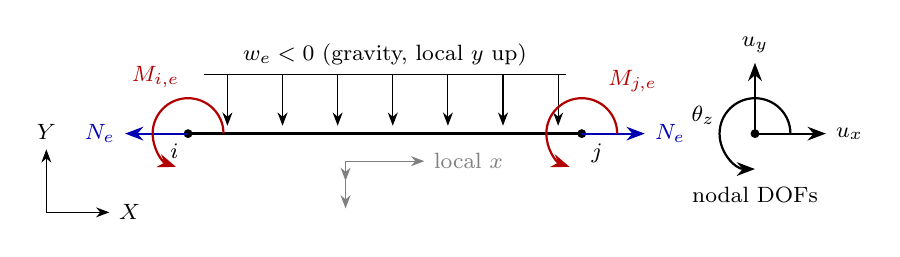
\begin{tikzpicture}[>=Stealth, font=\footnotesize, scale=1.0]
% global axes
\draw[->] (-0.6,-0.4) -- (0.2,-0.4) node[right]{$X$};
\draw[->] (-0.6,-0.4) -- (-0.6,0.4) node[above]{$Y$};
% member
\coordinate (I) at (1.2,0.6); \coordinate (J) at (6.2,0.6);
\draw[very thick] (I) -- (J);
\fill (I) circle (1.6pt) node[below left]{$i$}; \fill (J) circle (1.6pt) node[below right]{$j$};
\draw[->, gray] (3.2,0.25) -- (4.2,0.25) node[right]{local $x$};
\draw[->, gray] (3.2,0.25) -- (3.2,-0.35) node[below]{};
\draw[->, gray] (3.2,0.25) -- (3.2,0.0);
% distributed load
\foreach \x in {1.7,2.4,...,5.9} \draw[->] (\x,1.35) -- (\x,0.7);
\draw (1.4,1.35) -- (6.0,1.35); \node at (3.7,1.6) {$w_e<0$ (gravity, local $y$ up)};
% axial forces (tension positive)
\draw[->, thick, blue!70!black] (I) -- ++(-0.8,0) node[left]{$N_e$};
\draw[->, thick, blue!70!black] (J) -- ++(0.8,0) node[right]{$N_e$};
% end moments CCW
\draw[->, thick, red!70!black] ([shift={(0.45,0)}]I) arc (0:250:0.45) node[pos=0.35, above left]{$M_{i,e}$};
\draw[->, thick, red!70!black] ([shift={(0.45,0)}]J) arc (0:250:0.45) node[pos=0.25, above right]{$M_{j,e}$};
% node DOFs
\begin{scope}[shift={(8.4,0.6)}]
\fill (0,0) circle (1.6pt);
\draw[->, thick] (0,0) -- (0.9,0) node[right]{$u_x$};
\draw[->, thick] (0,0) -- (0,0.9) node[above]{$u_y$};
\draw[->, thick] (0.45,0) arc (0:270:0.45) node[pos=0.55, left]{$\theta_z$};
\node[below] at (0,-0.55) {nodal DOFs};
\end{scope}
\end{tikzpicture}
\caption{Sign conventions. Basic forces of member $e$ ($i\to j$): axial force $N_e$, tension positive; end moments $M_{i,e}$, $M_{j,e}$ acting on the member, counter-clockwise positive; transverse load $w_e$ along the local $y$ axis. Nodal displacements $u_x$, $u_y$ along the global axes and rotation $\theta_z$ counter-clockwise. Columns are oriented bottom to top, beams left to right.}\label{fig:signs}
\end{figure} This parametrisation satisfies member equilibrium identically \cite{mcguire2000matrix}. Rotating to global axes and assembling at the nodes gives the nodal equilibrium equations at the $n_f$ free degrees of freedom (DOFs),
\begin{equation}\label{eq:equilibrium}
\mathbf{C}\,\mathbf{q} = \mathbf{d}, \qquad \mathbf{C}\in\mathbb{R}^{n_f\times 3m},\quad \mathbf{d} = \mathbf{P}_f - \mathbf{p}^0_f ,
\end{equation}
where $\mathbf{q}$ stacks the basic forces of all $m$ members, $\mathbf{P}_f$ are the applied nodal loads and $\mathbf{p}^0_f$ the assembled particular solutions. $\mathbf{C}$ is the equilibrium (statics) matrix. For a kinematically stable frame it has full row rank and $3m-n_f$ equals the degree of static indeterminacy, so Eq.~\eqref{eq:equilibrium} defines an affine set of dimension $3m-n_f>0$ that contains the exact FE solution but also every other statically admissible force field. Equilibrium alone therefore cannot determine the forces, which is precisely why a learned prior is needed; conversely, any force prediction that violates Eq.~\eqref{eq:equilibrium} is mechanically inadmissible. Support reactions follow from $\mathbf{q}$ at the restrained DOFs, so a force field satisfying Eq.~\eqref{eq:equilibrium} also satisfies global equilibrium. Assembling $\mathbf{C}$ costs $\mathcal{O}(m)$ and requires no stiffness matrix.

\subsection{Dimensional analysis and exact load-case superposition}\label{sec:scaling}
For a linear elastic frame the response is linear in the loads. If $E$ is the same in every member, as here, the displacements and rotations are inversely proportional to $E$, whereas the member forces of this statically indeterminate structure depend only on the relative stiffnesses and are therefore independent of a uniform $E$. The surrogate imposes these properties exactly through dimensional analysis~\cite{buckingham1914pi}. Let $H=\frac{1}{n_s}\sum_s h_s$ be the mean storey height and $I_\mathrm{ref}=\frac{1}{n_s}\sum_s I_{c,s}$ the mean column second moment of area, so that $EI_\mathrm{ref}$ is a reference flexural rigidity. Each load case $c\in\{\mathrm{W},\mathrm{G}\}$ is scaled by its own intensity: the signed base shear $\lambda_\mathrm{W}=\sum_s F_s$ and the total gravity load $\lambda_\mathrm{G}=\sum_e |w_e|L_e$. The response is written as
\begin{equation}\label{eq:superposition}
\begin{aligned}
(u_x,u_y) &= \sum_{c} \frac{\lambda_c H^3}{EI_\mathrm{ref}}\,(\hat u_{x,c},\hat u_{y,c})(\boldsymbol{\pi}_c), &
\theta_z &= \sum_{c} \frac{\lambda_c H^2}{EI_\mathrm{ref}}\,\hat\theta_{c}(\boldsymbol{\pi}_c),\\
N &= \sum_c \lambda_c\, \hat N_c(\boldsymbol{\pi}_c), &
M &= \sum_c \lambda_c H\,\hat M_c(\boldsymbol{\pi}_c),
\end{aligned}
\end{equation}
where hats denote the network outputs and $\boldsymbol{\pi}_c$ is a set of dimensionless input groups (Table~\ref{tab:dimensions}): lengths divided by $H$, second moments of area divided by $I_\mathrm{ref}$, areas as $AH^2/I_\mathrm{ref}$, lateral loads divided by $\lambda_\mathrm{W}$ and gravity loads by $\lambda_\mathrm{G}$. Because $\boldsymbol{\pi}_c$ is invariant to the load magnitudes and to $E$, Eq.~\eqref{eq:superposition} is exactly homogeneous of degree one in each load-case intensity, the displacements scale exactly with $1/E$, the forces are exactly independent of a uniform $E$, and reversing the lateral load reverses the lateral response. $E$ does not appear in the force expressions at all, and $\lambda_c$ cancels in every input group.

In the generator, $|\lambda_\mathrm{W}|\ge 5$\,kN (all floor forces of a frame have the same sign) and $\lambda_\mathrm{G}>0$, so neither scale can vanish. In deployment a load case with $\lambda_c=0$ is simply omitted from the sum; a lateral pattern whose floor forces cancel ($\sum_sF_s\approx0$ but $\sum_s|F_s|>0$) would make $\lambda_\mathrm{W}$ ill-conditioned and should be scaled by $\sum_s|F_s|$ instead, a case that does not occur in this study and that the domain check of Section~\ref{sec:ood} would flag as unseen. Predicting the two cases separately also avoids a scaling problem: in the combined case the lateral sway is often orders of magnitude smaller than the gravity-induced quantities, so a single scale under-weights it. The ablation in Section~\ref{sec:ablation} quantifies this choice. Restrained DOFs are multiplied by zero, so the boundary conditions also hold exactly.

\begin{table}[t]
\centering
\caption{Dimensional consistency of the scaled formulation (units kN, m). Every input and output group of the network is dimensionless and independent of $\lambda_c$ and $E$.}\label{tab:dimensions}
\footnotesize
\begin{tabular}{llll}
\toprule
Quantity & Units & Scale & Dimensionless group \\
\midrule
Lengths $x$, $L$, $h$ & m & $H$ & $x/H$, $L/H$, $h/H$ \\
Second moment of area $I$ & m$^4$ & $I_\mathrm{ref}$ & $I/I_\mathrm{ref}$ \\
Cross-sectional area $A$ & m$^2$ & $I_\mathrm{ref}/H^2$ & $AH^2/I_\mathrm{ref}$ \\
Floor force $F_s$, storey shear $V_s$ & kN & $\lambda_\mathrm{W}$ & $F_s/\lambda_\mathrm{W}$, $V_s/\lambda_\mathrm{W}$ \\
Overturning moment & kN\,m & $\lambda_\mathrm{W}H$ & $\mathrm{OTM}/(\lambda_\mathrm{W}H)$ \\
Line load $w$ (resultant $wL$) & kN/m (kN) & $\lambda_\mathrm{G}$ & $wL/\lambda_\mathrm{G}$ \\
Drift estimate $\delta_s$ & m & $\lambda_\mathrm{W}H^3/EI_\mathrm{ref}$ & $\delta_s EI_\mathrm{ref}/(\lambda_\mathrm{W}H^3)$ \\
Displacements $u_x$, $u_y$ & m & $\lambda_cH^3/EI_\mathrm{ref}$ & $\hat u_{x,c}$, $\hat u_{y,c}$ \\
Rotation $\theta_z$ & rad & $\lambda_cH^2/EI_\mathrm{ref}$ & $\hat\theta_c$ \\
Axial force $N$ & kN & $\lambda_c$ & $\hat N_c$ \\
End moment $M$ & kN\,m & $\lambda_cH$ & $\hat M_c$ \\
Equilibrium rows (force / moment) & kN / kN\,m & $\lambda_c$ / $\lambda_cH$ & rows of $\mathbf{C}$, $\mathbf{d}_c$ \\
\bottomrule
\end{tabular}
\end{table}

\subsection{Mechanics-informed features}\label{sec:features}
Each node carries 25 dimensionless features and each member 10. Beyond position, topology and section ratios, they include two quantities from elementary statics that are exact and cost $\mathcal{O}(n)$, the storey shear $V_s=\sum_{k\ge s}F_k$ and the overturning moment of the loads above the storey, and three classical approximations. The first is the gravity load carried by each column line computed from tributary areas, i.e.\ as if every beam were simply supported; in a rigid frame continuity and sway redistribute these loads, so the feature is an approximation, not an exact statical quantity. The other two are the beam-to-column stiffness ratio of each storey, $\rho_s = (n_b I_{b,s}/\bar L_b)/((n_b+1)I_{c,s}/h_s)$, and the shear-building drift estimate $\delta_s = V_s/k_s$ with $k_s=(n_b+1)\,12EI_{c,s}/h_s^3$ (or $3EI/h^3$ for a pinned first storey), together with its height-wise cumulative sum. The network learns the correction from these simple estimates to the FE response, which is a smoother target than the response itself. The full feature dictionary with formulas is given in \ref{app:features}. The same features are given to all tabular baselines.

\subsection{Graph network}\label{sec:gnn}
Frames of different size and topology are represented as graphs whose nodes are joints and whose edges are members, and processed with an encode--process--decode message passing network~\cite{battaglia2018relational,gilmer2017mpnn,sanchez2020learning,pfaff2021meshgraphnets}. Node and edge features are encoded by two-layer perceptrons (width 96, SiLU, layer normalisation). Each of the eight processing steps updates every edge from its own state and the states of its end nodes, $\mathbf{z}_e \leftarrow \mathbf{z}_e + \phi_e([\mathbf{z}_e,\mathbf{h}_i,\mathbf{h}_j])$, and every node from the sums of the messages of the members that start and end at it, kept separate so that the network can distinguish the two ends of a member, $\mathbf{h}_i \leftarrow \mathbf{h}_i + \phi_n([\mathbf{h}_i,\sum_{e:i=\mathrm{start}}\mathbf{z}_e,\sum_{e:i=\mathrm{end}}\mathbf{z}_e])$. Eight steps nearly cover the graph diameter of the training frames (at most nine members), and frame-level information is supplied in addition through the statics features; the effect of the depth (4, 8, 12 and 16 steps) is examined in Section~\ref{sec:graphbaselines}. Decoders output six dimensionless displacements per node and six dimensionless basic forces per member (three per load case). The loss is the mean squared error of the outputs standardised per component, over free DOFs only. Training uses AdamW~\cite{loshchilov2019adamw} with a one-cycle learning-rate schedule (peak $2\times10^{-3}$), batches of 32 frames, gradient clipping at 1.0 and 150 epochs, implemented in PyTorch~\cite{paszke2019pytorch}. A variant with a soft equilibrium penalty $\|\mathbf{C}\hat{\mathbf{q}}_c-\mathbf{d}_c\|^2$ added to the loss is examined in the ablation.

\subsection{Equilibrium projection}\label{sec:projection}
A data-driven prediction $\hat{\mathbf{q}}$ will in general violate Eq.~\eqref{eq:equilibrium}. The proposed constraint layer replaces it with the closest statically admissible force field in a metric $\boldsymbol{\Sigma}^{-1}$:
\begin{equation}\label{eq:projection}
\mathbf{q}^\star = \arg\min_{\mathbf{C}\mathbf{q}=\mathbf{d}} (\mathbf{q}-\hat{\mathbf{q}})^{\mathsf T}\boldsymbol{\Sigma}^{-1}(\mathbf{q}-\hat{\mathbf{q}})
= \hat{\mathbf{q}} + \boldsymbol{\Sigma}\mathbf{C}^{\mathsf T}\left(\mathbf{C}\boldsymbol{\Sigma}\mathbf{C}^{\mathsf T}\right)^{-1}\left(\mathbf{d}-\mathbf{C}\hat{\mathbf{q}}\right),
\end{equation}
which follows from the Karush--Kuhn--Tucker conditions of the equality-constrained quadratic programme~\cite{nocedal2006numerical}. It is applied separately to each load case in dimensionless form. Two metrics are compared: the Euclidean metric on the dimensionless forces ($\boldsymbol{\Sigma}=\mathbf{I}$), and the \emph{variance-weighted} metric built from the ensemble variance $\sigma_k^2$ of each predicted dimensionless force component $k$ (Section~\ref{sec:uq}), so that the components the model is least sure of absorb most of the correction. Because an ensemble variance can be arbitrarily close to zero, the metric is regularised as
\begin{equation}\label{eq:sigmareg}
\boldsymbol{\Sigma}_\mathrm{reg} = \mathrm{diag}\!\left(\sigma_k^2 + \varepsilon\,\bar{\sigma}^2\right), \qquad \bar\sigma^2 = \frac{1}{3m}\sum_k \sigma_k^2,\quad \varepsilon = 10^{-6},
\end{equation}
per load case and frame; the floor makes $\boldsymbol{\Sigma}_\mathrm{reg}$ positive definite and scale-free. The system $(\mathbf{C}\boldsymbol{\Sigma}\mathbf{C}^{\mathsf T})\boldsymbol{\mu} = \mathbf{d}-\mathbf{C}\hat{\mathbf{q}}$ is solved by a dense LU factorisation with partial pivoting (LAPACK \texttt{gesv} through NumPy), so there is no iterative tolerance; the resulting equilibrium residuals are at round-off level (Section~\ref{sec:results}). The sensitivity of the results to $\varepsilon$, to the alternative floor $\mathrm{diag}(\max(\sigma_k^2,\varepsilon\bar\sigma^2))$ and the condition numbers of $\mathbf{C}\boldsymbol{\Sigma}\mathbf{C}^{\mathsf T}$ are reported in Section~\ref{sec:sensitivity}. If the prediction error were Gaussian, unbiased and independent between components with covariance $\boldsymbol{\Sigma}$, Eq.~\eqref{eq:projection} would be the posterior mean after conditioning on the equilibrium equations. The ensemble variance is at best a crude diagonal approximation of that covariance (the errors of neighbouring members are correlated and the ensemble under-represents the error under distribution shift), so this interpretation motivates the choice of metric but does not make $\mathbf{q}^\star$ a calibrated posterior.

\begin{proposition}\label{prop:projection}
Let $\mathbf{q}_\mathrm{FE}$ be the exact solution, so that $\mathbf{C}\mathbf{q}_\mathrm{FE}=\mathbf{d}$. For any prediction $\hat{\mathbf{q}}$ and any symmetric positive definite $\boldsymbol{\Sigma}$, the projected forces satisfy
$\|\mathbf{q}^\star-\mathbf{q}_\mathrm{FE}\|^2_{\boldsymbol{\Sigma}^{-1}} = \|\hat{\mathbf{q}}-\mathbf{q}_\mathrm{FE}\|^2_{\boldsymbol{\Sigma}^{-1}} - \|\hat{\mathbf{q}}-\mathbf{q}^\star\|^2_{\boldsymbol{\Sigma}^{-1}} \le \|\hat{\mathbf{q}}-\mathbf{q}_\mathrm{FE}\|^2_{\boldsymbol{\Sigma}^{-1}}$.
\end{proposition}
\begin{proof}
$\mathbf{q}^\star$ is the $\boldsymbol{\Sigma}^{-1}$-orthogonal projection of $\hat{\mathbf{q}}$ onto the affine set $\mathcal{A}=\{\mathbf{q}:\mathbf{C}\mathbf{q}=\mathbf{d}\}$. Since $\mathbf{q}^\star-\mathbf{q}_\mathrm{FE}$ lies in $\ker\mathbf{C}$ and $\hat{\mathbf{q}}-\mathbf{q}^\star=\boldsymbol{\Sigma}\mathbf{C}^{\mathsf T}\boldsymbol{\mu}$ for some $\boldsymbol{\mu}$, their $\boldsymbol{\Sigma}^{-1}$-inner product is $\boldsymbol{\mu}^{\mathsf T}\mathbf{C}(\mathbf{q}^\star-\mathbf{q}_\mathrm{FE})=0$, and the identity follows from Pythagoras' theorem.
\end{proof}
The projection can therefore never increase the error measured in its own metric, and it removes exactly the part of the error that is visible to statics. It does not guarantee a reduction of every individual component (for example the end moments alone), which is why the choice of metric matters and is examined empirically. The projection needs one dense solve of size $n_f$ per load case, which for the frames considered here takes a fraction of a millisecond, and it is model-agnostic: it is applied below to the baselines as well.

\subsection{Displacement--force compatibility}\label{sec:compat}
The network predicts displacements and forces with separate decoders, and the projection changes only the forces. The two fields are therefore not linked by the element stiffness relations. To measure this, the basic forces implied by the predicted displacements are computed member by member as $\mathbf{q}_\mathrm{const}(\hat{\mathbf{u}})$, i.e.\ the local end forces $\mathbf{k}_e\mathbf{T}_e\hat{\mathbf{u}}_e + \mathbf{f}^\mathrm{fix}_e$ (element stiffness $\mathbf{k}_e$, rotation $\mathbf{T}_e$ and fixed-end forces $\mathbf{f}^\mathrm{fix}_e$ of the member load), and the compatibility residual is defined as
\begin{equation}\label{eq:compat}
r_\mathrm{compat} = \frac{\|\mathbf{S}(\mathbf{q}-\mathbf{q}_\mathrm{const}(\hat{\mathbf{u}}))\|_2}{\|\mathbf{S}\,\mathbf{q}_\mathrm{const}(\hat{\mathbf{u}})\|_2},
\qquad r_{\mathrm{compat},M} = \frac{\|\mathbf{M}-\mathbf{M}_\mathrm{const}(\hat{\mathbf{u}})\|_2}{\|\mathbf{M}_\mathrm{const}(\hat{\mathbf{u}})\|_2},
\end{equation}
where $\mathbf{q}$ is the force field being assessed (raw, projected or recovered) and $\mathbf{S}$ divides the moment entries by $H$ so that forces and moments are commensurate. $r_{\mathrm{compat},M}$ uses the end moments only, because the axial forces implied by displacements, $EA/L$ times the member elongation, amplify small displacement errors by the large axial stiffness. A zero residual means that the forces are those the predicted displacements would produce; the exact FE solution has $r_\mathrm{compat}=0$ and zero equilibrium residual simultaneously. Recovering the forces from the predicted displacements, as in displacement-based surrogates~\cite{leng2026mcgnn}, gives $r_\mathrm{compat}=0$ by construction but sacrifices equilibrium; projecting the directly predicted forces gives exact equilibrium but leaves compatibility unenforced. Both options, and the effect of the projection on $r_\mathrm{compat}$, are quantified in Section~\ref{sec:compatresults}. A field that satisfies both conditions exactly is the FE solution itself; the predicted displacements can then serve as the initial iterate of an iterative solver, which is also examined.

\subsection{Predictive uncertainty}\label{sec:uq}
Epistemic uncertainty~\cite{derkiureghian2009aleatory} is estimated with a deep ensemble~\cite{lakshminarayanan2017ensembles} of $M=5$ networks that differ in initialisation and batch order and share the training data and normalisation. The ensemble mean is the prediction and the ensemble variance $\sigma^2$ of each output feeds the projection metric. For decisions at the level of a whole frame, the relative spread of the end moments,
\begin{equation}\label{eq:score}
s = \frac{\|\boldsymbol{\sigma}_M\|_2}{\|\hat{\mathbf{M}}\|_2},
\end{equation}
is used, where $\boldsymbol{\sigma}_M$ collects the physical standard deviations of all end moments. A second, label-free indicator is also examined: the equilibrium residual $\|\mathbf{C}\hat{\mathbf{q}}-\mathbf{d}\|/\|\mathbf{d}\|$ of the unprojected ensemble mean, which measures how far the raw prediction is from being statically admissible. The two indicators have different roles in the workflow. The ensemble spread $s$ is used at deployment, to decide whether an individual prediction is accepted or referred to the FE solver; the equilibrium residual is used during training, to decide which candidate frames are worth an FE analysis (Section~\ref{sec:workflow}).

\subsection{Domain check and calibrated referral threshold}\label{sec:ood}
An ensemble can be confidently wrong on inputs unlike its training data~\cite{ovadia2019shift}, and Section~\ref{sec:uqresults} shows that this happens for the unseen load patterns. The deployment rule therefore has two stages, both calibrated on the 400 ID validation frames, which are used neither for training nor for testing.

\emph{Stage 1: domain check.} Each frame is summarised by ten geometry descriptors (numbers of storeys and bays, largest storey height, first-to-mean storey height ratio, mean bay width, ratio of the largest to the smallest bay, height-to-width aspect ratio, $\log_{10}E$, $\log_{10}$ of the beam-to-column second-moment ratio, base fixity) and five load-pattern descriptors (normalised height of the centroid of the lateral forces, roof share of the lateral load, mean ratio of each beam load to the largest load on its floor, mean within-floor coefficient of variation of the beam loads, and $\log_{10}$ of the gravity-to-lateral load ratio). All are available before any analysis. The descriptors are standardised with the training-set statistics and the Mahalanobis distance~\cite{lee2018mahalanobis} to the training distribution is computed with a Ledoit--Wolf shrinkage covariance~\cite{ledoit2004shrinkage} estimated on the 3{,}000 training frames. A frame is outside the domain, and referred to FE, if its distance exceeds the 99th percentile of the distances of the validation frames (a nominal false-referral rate of 1\% for in-distribution frames). Distances based on the geometry and the load descriptors alone are also reported, to show which group detects which shift.

\emph{Stage 2: conformal error bound.} For frames inside the domain, the ensemble spread is converted into an error bound by split conformal prediction~\cite{lei2018conformal}. On the in-domain validation frames, the non-conformity scores $a_i = e_{M,i}/s_i$ (true moment error over spread) are computed and $\hat a$ is their $\lceil (n+1)(1-\alpha)\rceil$-th smallest value with $\alpha=0.1$. For a new frame the bound is $\hat a\,s$, which under exchangeability with the calibration frames covers the true moment error with probability at least $1-\alpha$. A frame is accepted if $\hat a\,s\le\tau$ for a tolerance $\tau$ on the relative moment error (5\% and 10\% are reported) and referred otherwise. Unlike the risk--coverage curves of Section~\ref{sec:uqresults}, which are computed on the test sets and serve only to describe the ranking quality, both thresholds of this rule are fixed before the test data are seen.

%% ---------------------------------------------------------------------------
\section{Uncertainty-guided workflow}\label{sec:workflow}

The surrogate is embedded in a workflow with two uses of the uncertainty estimate (Fig.~\ref{fig:workflow}).

\paragraph{Adaptive FE data generation} Training starts from $N_0$ randomly chosen frames of the candidate pool, analysed with PyNite. In each round an ensemble is trained, every remaining candidate is scored without any FE analysis, the $B$ highest-scoring candidates are analysed with PyNite and added to the training set. This is pool-based active learning~\cite{settles2009active} in the spirit of adaptive surrogate methods in structural reliability~\cite{bichon2008egra,echard2011akmcs}. Four acquisition rules are compared: random sampling, the ensemble variance (mean normalised variance over all outputs), the equilibrium residual of the raw prediction, and a diversity-aware variant of the latter. Selecting the $B$ largest scores can pick many near-identical frames from one corner of the design space, so the diversity-aware rule shortlists the $3B$ candidates with the largest residuals, groups them into $B$ clusters by $k$-means on standardised frame descriptors (the mean and maximum of the node features) and takes the highest-residual frame of each cluster, in the spirit of diverse mini-batch active learning~\cite{zhdanov2019diverse,sener2018coreset}. Each rule is repeated with five random initial sets (seeds 0--4). The candidates are labelled in advance for convenience, but a label is revealed to the learner only when the strategy requests that analysis, and the recorded PyNite time of each requested analysis is charged to the budget.

\paragraph{FE referral at deployment} For a batch of new frames, all are first predicted and projected. A frame is sent to PyNite, and its surrogate result discarded, if it fails the domain check or if its conformal error bound exceeds the tolerance (Section~\ref{sec:ood}); the remaining predictions are accepted. To describe how well the spread ranks the errors independently of any threshold, risk--coverage curves~\cite{geifman2017selective} are also reported, in which the fraction of frames with the largest spread referred to FE is varied.

\begin{figure}[t]
\centering
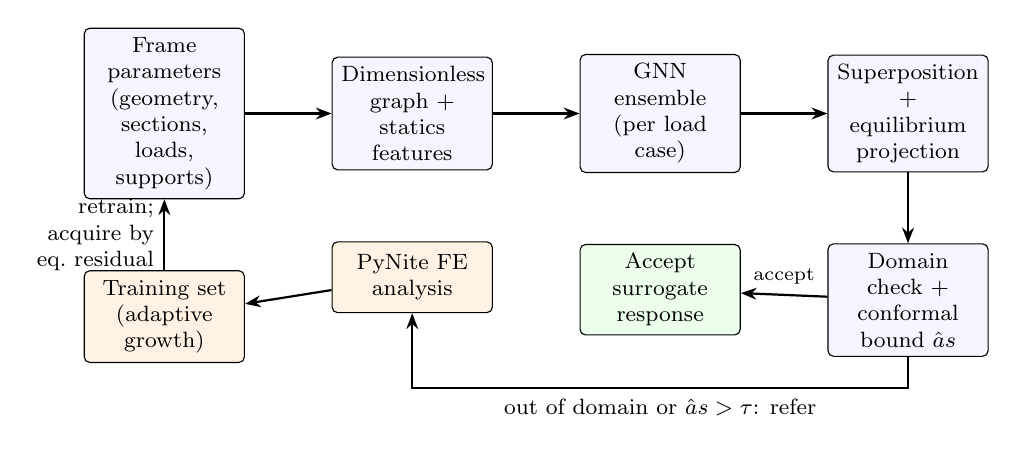
\begin{tikzpicture}[node distance=4mm and 11mm, every node/.style={font=\footnotesize, align=center},
  box/.style={draw, rounded corners=2pt, minimum height=9mm, text width=18mm, fill=blue!4},
  fe/.style={box, fill=orange!10}, arr/.style={-{Stealth[length=2mm]}, thick}]
\node[box] (param) {Frame parameters\\(geometry, sections,\\loads, supports)};
\node[box, right=of param] (feat) {Dimensionless\\graph + statics\\features};
\node[box, right=of feat] (gnn) {GNN ensemble\\(per load case)};
\node[box, right=of gnn] (proj) {Superposition +\\equilibrium\\projection};
\node[box, below=9mm of proj] (score) {Domain check +\\conformal bound $\hat a s$};
\node[box, below=9mm of gnn, fill=green!8] (accept) {Accept surrogate\\response};
\node[fe, below=9mm of feat] (fe) {PyNite FE\\analysis};
\node[fe, below=9mm of param] (train) {Training set\\(adaptive growth)};
\draw[arr] (param) -- (feat); \draw[arr] (feat) -- (gnn); \draw[arr] (gnn) -- (proj);
\draw[arr] (proj) -- (score);
\draw[arr] (score) -- node[above, font=\scriptsize]{accept} (accept);
\draw[arr] (score.south) -- ++(0,-4mm) -| node[pos=0.25, below]{out of domain or $\hat a s>\tau$: refer} (fe.south);
\draw[arr] (fe) -- (train);
\draw[arr] (train.north) -- node[left, align=right]{retrain;\\acquire by\\eq.\ residual} (param.south);
\end{tikzpicture}
\caption{Proposed workflow. Exact mechanics (superposition, boundary conditions, static equilibrium) is imposed around a learned graph ensemble. During training, new FE analyses are chosen by the equilibrium residual of the raw prediction; at deployment, a domain check and a conformal bound on the ensemble spread decide which frames are referred to PyNite.}\label{fig:workflow}
\end{figure}

%% ---------------------------------------------------------------------------
\section{Baselines and evaluation protocol}\label{sec:protocol}

\paragraph{Baselines} Five baselines represent conventional regression and widely used machine learning: ridge regression~\cite{hoerl1970ridge} on the features (linear) and on all their pairwise products (quadratic), random forests~\cite{breiman2001rf} (200 trees), histogram gradient boosting~\cite{friedman2001gbm} (600 iterations, one model per output) and a three-layer perceptron (256 units per layer, early stopping), all from scikit-learn~\cite{pedregosa2011sklearn}. Because fixed-length regressors cannot ingest graphs of varying size, they predict per node (displacements, from the 25 node features) and per member (basic forces, from the 10 member features concatenated with the features of both end nodes). They receive the same dimensionless, superposition-split targets and the same hard boundary conditions as the graph network, so that the comparison isolates the learning model and the constraint layer rather than the preprocessing. The quadratic ridge model is fitted on a random subset of 30{,}000 rows to keep the design matrix in memory. All models are trained on the same first 3{,}000 frames of the ID pool.

\paragraph{Graph-learning baselines}\label{sec:graphbaselinesdef} Five graph models isolate the design choices of the proposed network. All are trained on the same 3{,}000 frames for 150 epochs with three random seeds each.
(i) A \emph{conventional GNN}: the same architecture, but with physical inputs (coordinates, support flags, nodal loads, member length, $\log_{10}E$, $\log_{10}I$, $\log_{10}A$, line load) and physical targets for the combined load case, standardised over the training set; no statics features, no load-case split and no dimensional scaling.
(ii) A \emph{global-pooling} variant of the proposed network, in which the graph-wide mean of the node states is appended to every node update, giving every node frame-level context at every step.
(iii) A \emph{StructGNN-style} network following Chou et al.~\cite{chou2024structgnn}: one pseudo node per storey linked to all joints of that floor and to the pseudo node below, linear encoders to width 256, linear messages with mean aggregation in both edge directions, $n_s+1$ propagation steps for a frame with $n_s$ storeys (mini-batches grouped by $n_s$), decoders with one ReLU hidden layer and a mean-absolute-error loss. To allow a fair comparison it receives the same dimensionless features and targets as the proposed network. Two deviations from the original are needed: the weights are shared across propagation steps, because the unseen-geometry frames need up to nine steps whereas training frames need at most six, and a residual connection is added to train stably with the learning-rate schedule used for all models (the original used 1{,}000 epochs with batch size one, which was not affordable for all seeds here).
(iv) A \emph{displacement-only} network: the proposed architecture trained on the displacements only, with member forces recovered from the predicted displacements through the element stiffness relations and the fixed-end forces.
(v) A \emph{Leng-style} network following Leng et al.~\cite{leng2026mcgnn}: as (iv), with the normalised free-DOF stiffness residual $\|\mathbf{K}_{ff}\hat{\mathbf{u}}_f-\mathbf{f}_f\|^2/\|\mathbf{f}_f\|^2$ added to the loss with weight $10^{-2}$, chosen from $\{10^{-4},10^{-3},10^{-2},10^{-1},1\}$ on a short pilot run because larger weights let the poorly conditioned axial rows dominate. These are re-implementations from the published descriptions, not the authors' code.
The soft-equilibrium-penalty and no-superposition ablations of the proposed network and a depth ablation (4, 8, 12, 16 message-passing steps) are trained with three seeds as well.

\paragraph{Metrics} All errors are computed per frame in physical units against PyNite and summarised over a test set by the median and the 95th percentile (p95). With $\hat{\cdot}$ the surrogate and $\|\cdot\|$ the Euclidean norm over all entries of a frame, the field errors are relative $L_2$ errors, $e_a = \|\hat{\mathbf{a}}-\mathbf{a}\|/\|\mathbf{a}\|$, for the horizontal displacements ($e_{u_x}$), vertical displacements ($e_{u_y}$) and rotations ($e_\theta$) of all nodes, the end moments ($e_M$), axial forces ($e_N$) and end shears ($e_V$) of all members, and the support reactions ($e_R$). The peak-response errors are $|\max\hat a-\max a|/\max a$ for the largest inter-storey drift ratio ($e_\mathrm{drift}$), the largest beam mid-span deflection relative to the chord ($e_\mathrm{defl}$; Hermite interpolation of the end rotations plus the fixed-end deflection $wL^4/(384EI)$), the largest absolute end moment ($e_{M,\max}$) and the largest absolute axial force ($e_{N,\max}$). The governing-member agreement is the fraction of frames in which the member with the largest end moment is predicted as the largest (top-1) or among the three largest (top-3). The equilibrium residual is $\|\mathbf{r}\|/\|\mathbf{P}_f-\mathbf{p}^0_f\|$ with $\mathbf{r}$ the nodal out-of-balance force at the free DOFs, moment rows divided by $H$; the compatibility residual is Eq.~\eqref{eq:compat}.

\paragraph{Statistics} The proposed ensemble is trained five times independently (five ensembles of five networks, 25 networks in total, with disjoint seeds). For each metric the per-run median and p95 are reported as mean $\pm$ standard deviation over the five runs, with a 95\% confidence interval from the $t$ distribution with four degrees of freedom. Within one run, 95\% confidence intervals of the median and p95 over test frames are obtained by the percentile bootstrap~\cite{efron1993bootstrap} with 2{,}000 resamples, and differences between two variants evaluated on the same frames (e.g.\ raw versus projected forces) by a paired bootstrap. Graph baselines are reported as mean $\pm$ standard deviation over three seeds and tabular baselines with bootstrap intervals.

\paragraph{Computing environment} All experiments ran on a cloud virtual machine with four cores of an Intel Xeon processor at 2.1\,GHz, 15\,GB of memory and no GPU, under Linux with Python 3.13, PyNite 3.2.0, NumPy 2.5, SciPy 1.18, scikit-learn 1.9, PyTorch 2.15 and OpenSeesPy 3.8. Networks were trained on the CPU with one thread each, four in parallel; timing measurements were taken separately on the otherwise idle machine (Section~\ref{sec:cost}).

%% ---------------------------------------------------------------------------
\section{Results}\label{sec:results}

All numbers in this section are produced by the released scripts. Unless stated otherwise, errors are medians over the frames of a test set (600 frames for ID, OOD-G and OOD-L, 300 for DES), the proposed surrogate is the five-network ensemble with variance-weighted projection, and single numbers refer to the first of five independent training runs (ensemble 0); the variation over the five runs is reported in Section~\ref{sec:stats}.

\begin{figure}[p]
\centering
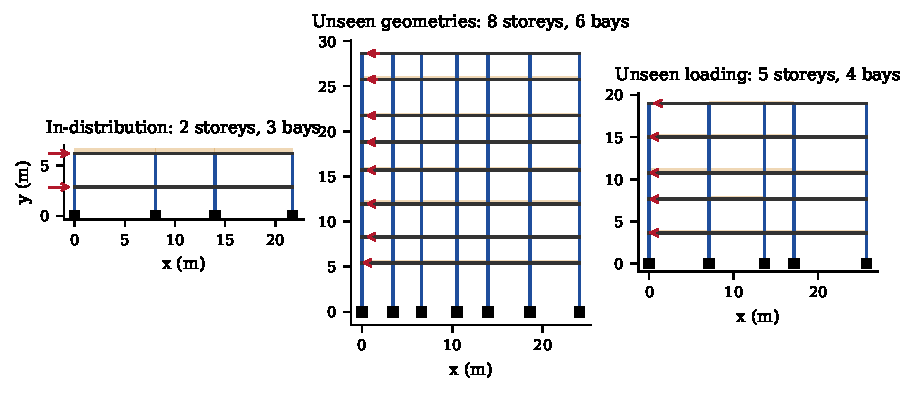
\includegraphics[width=\textwidth]{fig_frames.pdf}
\caption{Example frames from the four test sets. Blue: columns; black: beams; shaded: gravity line loads (scaled); red arrows: lateral floor forces; squares and triangles: fixed and pinned bases.}\label{fig:frames}
\end{figure}

\subsection{Dataset}
The 5{,}000-frame pool contains frames with 3 to 45 members (18 on average), the OOD-G set frames with 11 to 104 members (56 on average) and the DES set frames with 3 to 45 members (18 on average); Fig.~\ref{fig:frames} shows one frame of each set. A PyNite analysis of one frame (both load cases, including model construction and result extraction) took 37.5\,ms on average for the ID frames and 104.7\,ms for the larger OOD-G frames (Section~\ref{sec:cost}). Because sections and loads of the ID, OOD-G and OOD-L frames are sampled independently and are not sized for serviceability, the median largest inter-storey drift ratio is 0.46\% (ID) and 0.79\% (OOD-G), and 15\% and 25\% of these frames exceed 2\%. The design-driven frames are stiffer, with a median largest drift ratio of 0.18\%; 29\% of them exceed $h/400$ because the column sizing uses a simplified shear-building estimate. Since all models predict dimensionless responses that are exactly invariant to the load intensities and to $E$ (Section~\ref{sec:scaling}), the relative errors reported below do not depend on the load magnitudes.

\subsection{Accuracy on seen and unseen frames}\label{sec:accuracy}

\begin{table}[p]
\centering
\caption{Prediction errors on the in-distribution and design-driven test sets (medians over the frames, in \%, except the 95th percentile (p95) of $e_M$; last column: median relative nodal out-of-balance force). Bold: best value per column and set. The last row of each block gives the proposed surrogate as mean $\pm$ standard deviation of the per-run values over five independent training runs.}\label{tab:main}
\footnotesize
\setlength{\tabcolsep}{4pt}
\begin{adjustbox}{max width=\textwidth}
\begin{tabular}{lrrrrrr}
\toprule
Model & $e_{u_x}$ & $e_\mathrm{drift}$ & $e_M$ & $e_M$ (p95) & $e_N$ & Out-of-balance \\
\midrule
\inputtable{tables/tab_main_a.tex}
\bottomrule
\end{tabular}
\end{adjustbox}
\end{table}

\begin{table}[p]
\centering
\caption{As Table~\ref{tab:main}, for the unseen-geometry and unseen-loading test sets.}\label{tab:mainood}
\footnotesize
\setlength{\tabcolsep}{4pt}
\begin{adjustbox}{max width=\textwidth}
\begin{tabular}{lrrrrrr}
\toprule
Model & $e_{u_x}$ & $e_\mathrm{drift}$ & $e_M$ & $e_M$ (p95) & $e_N$ & Out-of-balance \\
\midrule
\inputtable{tables/tab_main_b.tex}
\bottomrule
\end{tabular}
\end{adjustbox}
\end{table}

Tables~\ref{tab:main} and~\ref{tab:mainood} compare the proposed surrogate with the five tabular baselines, and Fig.~\ref{fig:cdf} shows the full error distributions. On the in-distribution test set the proposed surrogate reaches median errors of 4.5\% for the horizontal displacement field, 4.9\% for the governing drift ratio, 2.4\% for the end-moment field and 0.6\% for the axial forces. The best baseline, gradient boosting, has 29.0\%, 30.2\%, 10.0\% and 3.2\%, so the graph surrogate is about four times more accurate for the member forces and six times more accurate for the displacements, although the baselines receive the same mechanics-informed features, targets and boundary conditions. The gap is largest for displacements, which depend on the stiffness of the whole frame and not only on local quantities. The design-driven frames, whose parameter correlations were never seen in training, are predicted as accurately as the ID frames: median errors of 4.4\% ($u_x$), 3.0\% (drift) and 2.0\% (moments), with a 95th percentile of the moment error of only 3.4\%, against 8.7\% (moments) and 37\% ($u_x$) for the best baselines.

\begin{figure}[p]
\centering
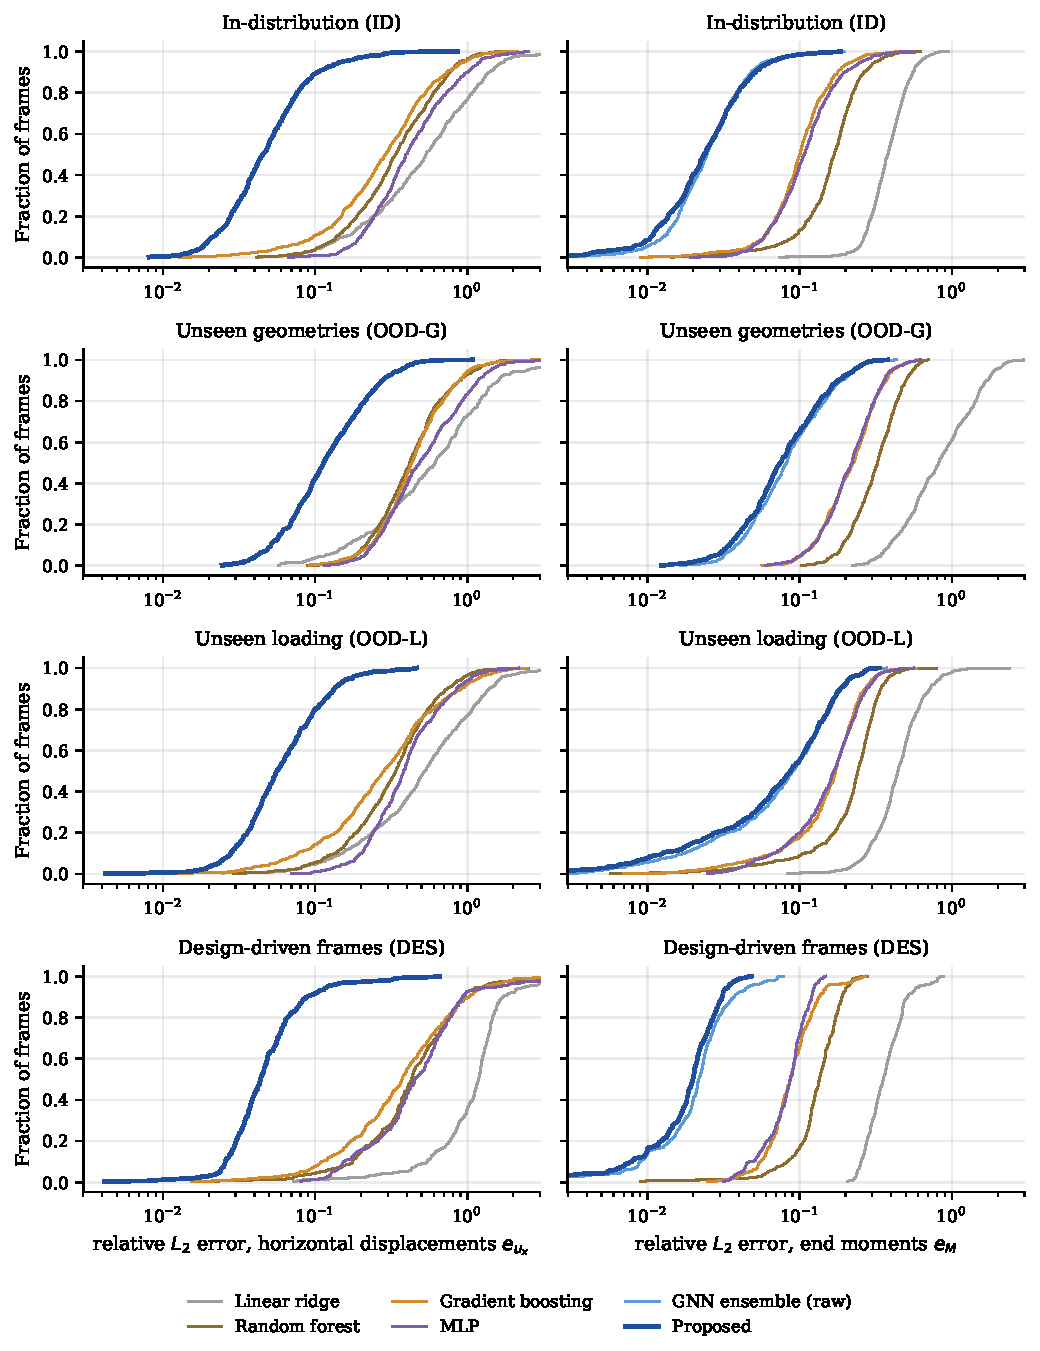
\includegraphics[width=\textwidth]{fig_error_cdf.pdf}
\caption{Cumulative distributions of the per-frame relative errors of the horizontal displacement field (left) and of the end-moment field (right) for the four test sets.}\label{fig:cdf}
\end{figure}

All models lose accuracy on the unseen geometries and load patterns, but the ranking is unchanged. For unseen geometries (up to eight storeys and six bays, against at most five and four in training) the proposed surrogate has a median moment error of 7.5\% and a median displacement error of 11.4\%, against 22.5\% and 43.1\% for gradient boosting; the governing-drift error is 13.7\%, whereas the tabular baselines have errors of 72--143\%. For unseen load patterns the median moment error is 8.7\% (gradient boosting 17.3\%, MLP 16.8\%) and the displacement error 5.6\%. The tails are heavy: the 95th percentile of the moment error is 22.6\% for unseen geometries and 21.4\% for unseen loading, which is not acceptable for design without further checks and motivates the referral rule of Section~\ref{sec:uqresults}. Figure~\ref{fig:parity} shows parity plots for the roof displacement and the largest end moment, and Fig.~\ref{fig:example} the end moments of a typical unseen-geometry frame.

\begin{table}[t]
\centering
\caption{Extended response metrics of the proposed surrogate: median and 95th percentile (p95) of the per-frame errors (\%), mean $\pm$ standard deviation over five independent training runs. Governing member: share of frames in which the member with the largest end moment is predicted as the largest (top-1) or among the three largest (top-3).}\label{tab:extended}
\footnotesize
\setlength{\tabcolsep}{3pt}
\begin{adjustbox}{max width=\textwidth}
\begin{tabular}{lrrrrrrrr}
\toprule
& \multicolumn{2}{c}{ID} & \multicolumn{2}{c}{OOD-G} & \multicolumn{2}{c}{OOD-L} & \multicolumn{2}{c}{DES}\\
\cmidrule(lr){2-3}\cmidrule(lr){4-5}\cmidrule(lr){6-7}\cmidrule(lr){8-9}
Metric & median & p95 & median & p95 & median & p95 & median & p95\\
\midrule
\inputtable{tables/tab_extended.tex}
\bottomrule
\end{tabular}
\end{adjustbox}
\end{table}

Table~\ref{tab:extended} extends the evaluation to the quantities an engineer checks. Vertical displacements and rotations are predicted with median errors of 3.2\% and 4.2\% on ID frames. The largest beam mid-span deflection, the largest end moment and the largest axial force, which govern serviceability and member design, are within 0.6\%, 0.8\% and 0.2\% of PyNite at the median, and the support reactions within 0.6\%; the 95th percentiles of these peak quantities stay below 4.5\% on the ID and DES sets. End shears follow the moments (median 1.2\%). The member with the largest end moment is identified correctly in about 94\% of the ID frames and is among the three predicted largest in almost all frames. On the unseen sets the peak quantities degrade much less than the full fields (largest moment 2.2\% and 2.5\% at the median for OOD-G and OOD-L), whereas the rotations and the governing drift ratio show the largest tails (95th percentiles of 28--40\% for the rotations and up to 97\% for the governing drift on OOD-G), so serviceability checks on unseen frames are the least reliable use of the surrogate.

\begin{figure}[p]
\centering
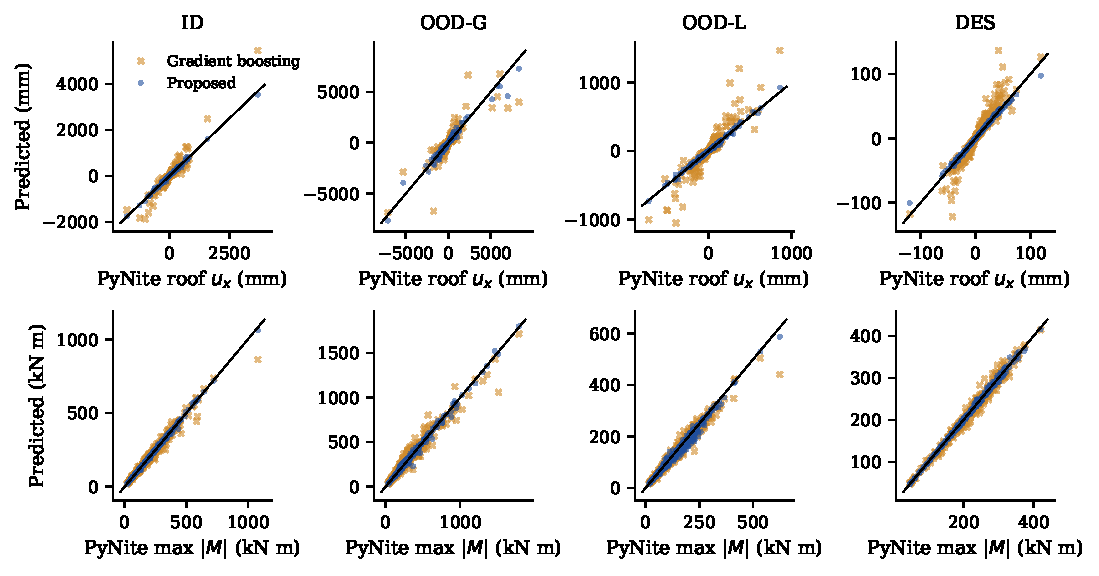
\includegraphics[width=\textwidth]{fig_parity.pdf}
\caption{Predicted versus PyNite roof displacement (top; mean of the roof nodes) and largest absolute end moment (bottom) for the proposed surrogate and the best tabular baseline.}\label{fig:parity}
\end{figure}

\begin{figure}[t]
\centering
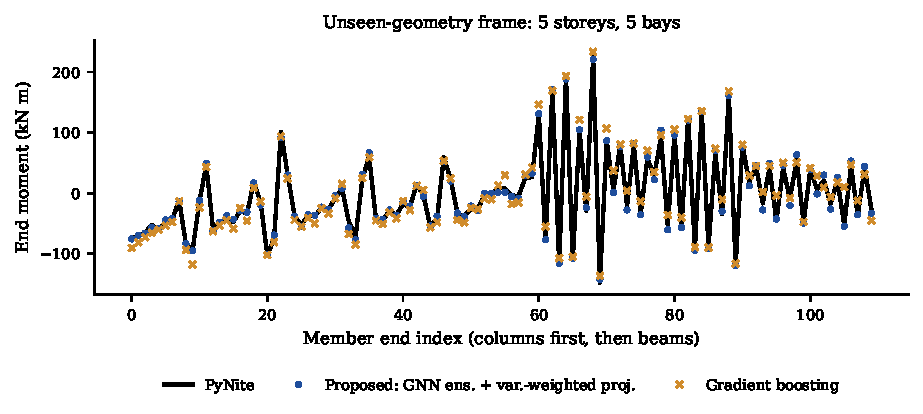
\includegraphics[width=\textwidth]{fig_example.pdf}
\caption{End moments of all members of an unseen-geometry frame (the OOD-G frame with the median number of members): PyNite, proposed surrogate and gradient boosting.}\label{fig:example}
\end{figure}

\subsection{Statistical robustness}\label{sec:stats}

\begin{table}[t]
\centering
\caption{Uncertainty of the headline results (moment error $e_M$, \%). Bootstrap: 95\% percentile-bootstrap interval over test frames for ensemble 0 (2{,}000 resamples). Across runs: mean and 95\% $t$-interval of the per-run median over five independent ensembles. Raw $-$ projected: reduction of the median $e_M$ by the variance-weighted projection, paired bootstrap for ensemble 0 and $t$-interval over the five runs.}\label{tab:stats}
\footnotesize
\begin{adjustbox}{max width=\textwidth}
\begin{tabular}{lccccc}
\toprule
Set & Median (bootstrap) & p95 (bootstrap) & Median (across runs) & Raw $-$ proj.\ (bootstrap) & Raw $-$ proj.\ (across runs)\\
\midrule
\inputtable{tables/tab_stats.tex}
\bottomrule
\end{tabular}
\end{adjustbox}
\end{table}

The five independent training runs (25 networks) give almost the same errors (Tables~\ref{tab:main}--\ref{tab:stats}): the per-run median moment error is $2.37\pm0.03\%$ (ID), $7.65\pm0.24\%$ (OOD-G), $8.79\pm0.32\%$ (OOD-L) and $1.99\pm0.08\%$ (DES), and the median displacement error $4.45\pm0.15\%$, $12.1\pm0.5\%$, $5.85\pm0.15\%$ and $4.45\pm0.12\%$. The variation between runs is much smaller than the sampling uncertainty of a single run over the test frames: the 95\% bootstrap interval of the ID median moment error of ensemble 0 is [2.24, 2.52]\%, and that of the 95th percentile [5.8, 7.2]\%. Every difference between the proposed surrogate and the tabular baselines in Tables~\ref{tab:main}--\ref{tab:mainood} is far larger than these intervals.

The effect of the projection on the median moment error is small and must be read with its intervals. On the ID set it lowers the median by 0.10 percentage points (2.46\%$\to$2.36\% for ensemble 0). The reduction has the same sign in all five runs (95\% $t$-interval [0.05, 0.14] points), but the paired bootstrap interval for a single run, [$-0.01$, 0.20] points, includes zero. The reduction is larger and significant in both senses on unseen geometries (0.53 points across runs, [0.33, 0.72]) and on the DES set (0.17, [0.08, 0.26]); on unseen load patterns the across-run interval includes zero. The projection should therefore be credited with exact equilibrium and a large reduction of the axial-force errors (Section~\ref{sec:eqresults}), and with a modest, consistent reduction of the moment errors, not with a decisive gain in moment accuracy.

\subsection{Graph-learning baselines, ablations and message-passing depth}\label{sec:graphbaselines}\label{sec:ablation}

\begin{table}[p]
\centering
\caption{Single graph networks (no ensembling, no projection): median $e_{u_x}$ and $e_M$ (\%), mean $\pm$ standard deviation over three training seeds. All models are trained on the same 3{,}000 frames for 150 epochs.}\label{tab:graph}
\footnotesize
\setlength{\tabcolsep}{3pt}
\begin{adjustbox}{max width=\textwidth}
\begin{tabular}{lrrrrrrrr}
\toprule
& \multicolumn{2}{c}{ID} & \multicolumn{2}{c}{OOD-G} & \multicolumn{2}{c}{OOD-L} & \multicolumn{2}{c}{DES}\\
\cmidrule(lr){2-3}\cmidrule(lr){4-5}\cmidrule(lr){6-7}\cmidrule(lr){8-9}
Model & $e_{u_x}$ & $e_M$ & $e_{u_x}$ & $e_M$ & $e_{u_x}$ & $e_M$ & $e_{u_x}$ & $e_M$\\
\midrule
\inputtable{tables/tab_graph.tex}
\bottomrule
\end{tabular}
\end{adjustbox}
\end{table}

\begin{table}[t]
\centering
\caption{Equilibrium and compatibility of the graph baselines (single networks, mean of three seeds): median relative out-of-balance force of the raw forces, median $e_M$ (\%) after Euclidean projection of the forces, median moment compatibility residual $r_{\mathrm{compat},M}$ (\%), and training time of one network on one CPU thread (min).}\label{tab:grapheq}
\footnotesize
\setlength{\tabcolsep}{3pt}
\begin{adjustbox}{max width=\textwidth}
\begin{tabular}{lrrrrrrr}
\toprule
& \multicolumn{3}{c}{ID} & \multicolumn{3}{c}{OOD-G} & \\
\cmidrule(lr){2-4}\cmidrule(lr){5-7}
Model & Eq.\ res. & $e_M$ proj. & $r_{\mathrm{compat},M}$ & Eq.\ res. & $e_M$ proj. & $r_{\mathrm{compat},M}$ & Train (min)\\
\midrule
\inputtable{tables/tab_graph_eq.tex}
\bottomrule
\end{tabular}
\end{adjustbox}
\end{table}

Table~\ref{tab:graph} compares single networks, so that the architecture is separated from the ensemble and the projection. Four findings stand out.

\emph{Mechanics-informed inputs and the load-case split matter more than the architecture.} The conventional GNN with physical inputs and targets has more than twice the displacement error of the proposed network on ID frames (14.3\% against 6.7\%) and 2.4--3.9 times on the unseen and design-driven sets, and 1.5 times the moment error on ID and OOD-G frames, although its moment error on unseen load patterns is lower (8.4\% against 10.0\%). Replacing the load-case split by a single combined load scale roughly doubles the displacement errors (12.5\% ID, 26.0\% OOD-G, 34.9\% DES) and raises the moment errors by up to 3.5 points (OOD-L unchanged), confirming the scaling argument of Section~\ref{sec:scaling}: in the combined case the lateral sway is masked by the much larger gravity scale.

\emph{The StructGNN-style network is a strong competitor.} With the same inputs and targets it reaches displacement errors similar to or lower than the proposed network (6.3\% ID, 12.3\% OOD-G, 7.1\% OOD-L) and slightly higher moment errors on ID, OOD-G and DES frames (4.2\%, 11.9\% and 3.9\% against 3.7\%, 11.3\% and 3.3\%); on unseen load patterns it is marginally better (9.7\% against 10.0\%). Its storey pseudo nodes and height-dependent depth carry global information quickly, which helps the displacements, at seven times the training cost (77 against 11 minutes per network on one thread). The proposed network with global pooling or with 16 message-passing steps gains in the same way (OOD-G displacement error 11.1\% and 11.8\% against 14.1\%) at little or no cost in moment accuracy. The accuracy of a single network is therefore not what distinguishes the proposed framework; the distinguishing elements are the exact constraints, the uncertainty estimate and its use, which are evaluated in the following sections and could equally be wrapped around a StructGNN-style network.

\emph{Depth mainly affects the displacements} (Fig.~\ref{fig:depth}). Going from 4 to 8 message-passing steps reduces the median displacement error from 9.1\% to 6.7\% (ID) and from 20.1\% to 14.1\% (OOD-G); 12 and 16 steps reduce it further to 5.8\% and 11.8\% (16 steps), whereas the moment errors improve from 4 to 8 steps (4.2\%$\to$3.7\% ID) and change by at most 0.1 points beyond 8 steps. Displacements depend on the stiffness of the whole frame and benefit from information travelling across the full graph diameter (up to 14 members in the OOD-G frames, against 9 in training), while end moments are governed mainly by the neighbourhood of the member and by the statics features. Eight steps were kept for the main model because they halve the training cost of 16 steps and the ensemble recovers most of the difference (ensemble displacement error 4.5\% ID, 11.4\% OOD-G).

\emph{Displacement-based force recovery is much less accurate than predicting forces directly.} A network trained on displacements alone has displacement errors close to the proposed network (7.4\% ID), but the forces recovered from its displacements have median moment errors of 20\% (ID) and 75\% (OOD-G), and their out-of-balance force exceeds the applied load (Table~\ref{tab:grapheq}). Adding the stiffness residual to the loss in the Leng-style variant did not help in our implementation: at a weight of $10^{-2}$ the residual term dominates and the displacement errors rise to 48\% (ID), and at $10^{-4}$ they are still 14\%, with moment errors of 30\% (ID). The free-DOF residual is dominated by the axial rows, whose stiffness exceeds the flexural stiffness by orders of magnitude, so penalising it pulls the network towards axial compatibility at the expense of the flexural response. A carefully scaled residual (for example, row-scaled by the diagonal of $\mathbf{K}$) may perform better, and this result should not be read as a verdict on the original method, whose code we did not use. Finally, the soft equilibrium penalty neither improves accuracy nor materially reduces the out-of-balance force (6.2\% against 6.7\% on ID frames), which supports enforcing equilibrium exactly instead of through the loss.

\begin{figure}[t]
\centering
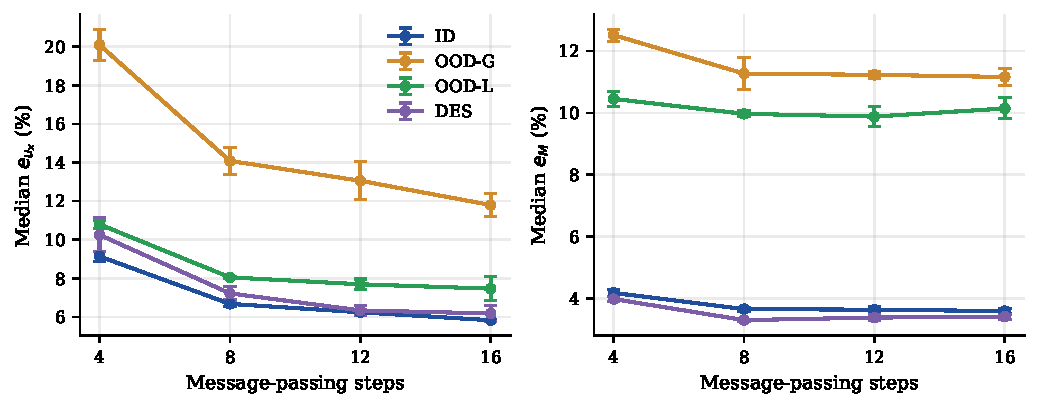
\includegraphics[width=\textwidth]{fig_depth.pdf}
\caption{Effect of the number of message-passing steps on the median displacement (left) and moment (right) errors of single networks (mean $\pm$ standard deviation over three seeds).}\label{fig:depth}
\end{figure}

\subsection{Equilibrium and the projection layer}\label{sec:eqresults}
Without the projection, every model produces member forces that are not in equilibrium with the applied loads (Fig.~\ref{fig:equilibrium}). The median out-of-balance force is 4\% of the load vector for the raw graph ensemble and 7--43\% for the tabular baselines on in-distribution frames, rising to 16\% and 18--120\% for unseen geometries. After projection (Eq.~\ref{eq:projection}) the residual is below $10^{-12}$ for every frame and every model, so the support reactions balance the loads and every nodal free body is in equilibrium.

\begin{figure}[t]
\centering
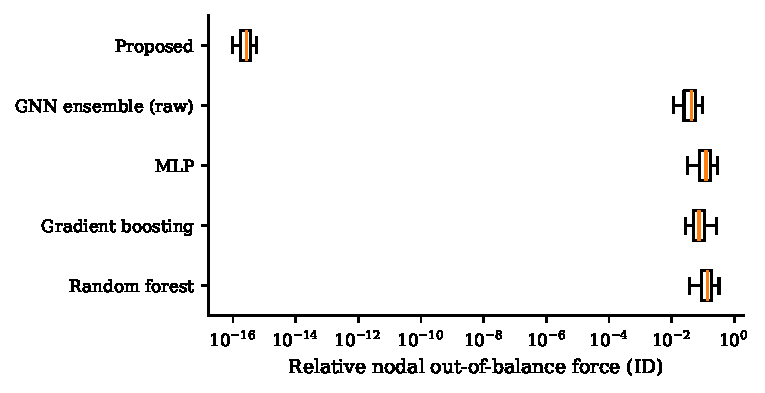
\includegraphics[width=0.75\textwidth]{fig_equilibrium.pdf}
\caption{Relative nodal out-of-balance force of the predicted member forces on the in-distribution test set (box: quartiles; whiskers: 5th--95th percentiles). Only the projected surrogate is statically admissible.}\label{fig:equilibrium}
\end{figure}

The metric of the projection matters. With the variance-weighted metric the axial-force error decreases by a factor of 2--4.7 (1.8\%$\to$0.6\% ID, 5.3\%$\to$1.5\% OOD-G, 3.5\%$\to$1.6\% OOD-L, 1.4\%$\to$0.3\% DES; Table~\ref{tab:compat}), the support-reaction errors by a factor of 2--3.5, and the moment errors decrease modestly (Section~\ref{sec:stats}). With the Euclidean metric the projection degrades the moments (2.5\%$\to$4.0\% ID, 8.3\%$\to$12.6\% OOD-G) while still improving the axial forces. This is consistent with Proposition~\ref{prop:projection}: the error can only decrease in the metric of the projection, and the Euclidean metric on dimensionless forces lets the correction flow into the moments, whose uncertainty it ignores.

\begin{table}[t]
\centering
\caption{Effect of the Euclidean equilibrium projection on the tabular baselines: median moment error $e_M$ and axial-force error $e_N$ (\%) before $\to$ after projection.}\label{tab:projbase}
\footnotesize
\setlength{\tabcolsep}{3pt}
\begin{adjustbox}{max width=\textwidth}
\begin{tabular}{lrrrrrrrr}
\toprule
& \multicolumn{2}{c}{ID} & \multicolumn{2}{c}{OOD-G} & \multicolumn{2}{c}{OOD-L} & \multicolumn{2}{c}{DES}\\
\cmidrule(lr){2-3}\cmidrule(lr){4-5}\cmidrule(lr){6-7}\cmidrule(lr){8-9}
Model & $e_M$ & $e_N$ & $e_M$ & $e_N$ & $e_M$ & $e_N$ & $e_M$ & $e_N$\\
\midrule
\inputtable{tables/tab_proj_baselines.tex}
\bottomrule
\end{tabular}
\end{adjustbox}
\end{table}

Because the layer is model-agnostic, it was also applied to the tabular baselines (Table~\ref{tab:projbase}), which provide no per-output variance, so the Euclidean metric is used. The axial-force errors decrease for every baseline and test set. The moment errors decrease for gradient boosting and for the MLP on most sets, but increase for the linear ridge model and the random forest; in the conventional GNN, whose Euclidean metric acts on physical forces, the projection reduces the moment errors (5.4\%$\to$4.4\% ID, 16.9\%$\to$12.7\% OOD-G), whereas for the dimensionless single networks it increases them (Table~\ref{tab:grapheq}). The projection therefore always delivers admissible forces and always improves the axial forces, while its effect on the moments depends on whether the metric reflects where the prediction errors actually are, which is what the ensemble variance provides.

\subsection{Displacement--force compatibility}\label{sec:compatresults}

\begin{table}[t]
\centering
\caption{Equilibrium and compatibility of the force fields of the proposed ensemble (ensemble 0): medians over the test frames (\%, residuals as fractions). $r_\mathrm{compat}$ and $r_{\mathrm{compat},M}$: Eq.~\eqref{eq:compat}; eq.\ res.: relative nodal out-of-balance force. The displacements are the same in all rows.}\label{tab:compat}
\footnotesize
\begin{adjustbox}{max width=\textwidth}
\begin{tabular}{lrrrrrr}
\toprule
Force field & $e_M$ & $e_N$ & $e_V$ & Eq.\ res. & $r_\mathrm{compat}$ & $r_{\mathrm{compat},M}$ \\
\midrule
\inputtable{tables/tab_compat.tex}
\bottomrule
\end{tabular}
\end{adjustbox}
\end{table}

Table~\ref{tab:compat} answers the question whether the projection makes the force field more or less compatible with the predicted displacements. The forces implied by the predicted displacements differ substantially from the predicted forces: the median compatibility residual of the raw ensemble is 47\% on the ID set and 87\% on unseen geometries. Most of this comes from the axial forces, because a displacement error of a few per cent, multiplied by the large axial stiffness $EA/L$, produces axial forces that are far from the true ones; restricted to the end moments the residual is 11\% (ID), 40\% (OOD-G), 18\% (OOD-L) and 4\% (DES). The equilibrium projection hardly changes these numbers. With the variance-weighted metric, $r_{\mathrm{compat},M}$ increases in 68\%, 67\%, 74\% and 69\% of the ID, OOD-G, OOD-L and DES frames, but only by a median factor of 1.01--1.04; with the Euclidean metric the increase is larger (median factor 1.03--1.34) and affects 82--93\% of the frames. The projection therefore slightly increases the incompatibility, as expected for a correction that acts on the forces alone, and the size of the increase follows the size of the force correction.

Recovering the forces from the predicted displacements, as in displacement-based surrogates~\cite{leng2026mcgnn}, gives zero compatibility residual by construction, but much less accurate forces and large equilibrium violations: the median moment error rises from 2.4\% to 11.2\% (ID) and from 7.5\% to 44.2\% (OOD-G), the axial-force errors reach 53\% and 183\%, and the out-of-balance force exceeds the applied load (median residual 1.7 and 9.8). Member forces are second derivatives of the displacement field, so the differentiation amplifies the displacement errors. In this setting, predicting the forces directly and imposing equilibrium is far more accurate than imposing compatibility, which is why the proposed workflow enforces the former and only measures the latter. A field that satisfies both is the FE solution. Using the predicted displacements as the starting point of a Jacobi-preconditioned conjugate-gradient solve of the full stiffness equations did not reduce the number of iterations to a relative residual of $10^{-8}$ (median 27 iterations for ID frames with and without the warm start; 72 for OOD-G), because the initial residual is dominated by the stiff axial DOFs: at the median it is 1.4 times (ID) and 12 times (OOD-G) the norm of the load vector, i.e.\ larger than the residual of a zero initial guess. A compatibility-aware correction that would help in practice would have to treat the axial and flexural parts separately and is left for future work.


\subsection{Sensitivity of the projection to the variance floor}\label{sec:sensitivity}

\begin{table}[t]
\centering
\caption{Sensitivity of the variance-weighted projection to the regularisation of $\boldsymbol{\Sigma}$ (ensemble 0): median moment error $e_M$ (\%) and largest condition number of $\mathbf{C}\boldsymbol{\Sigma}\mathbf{C}^{\mathsf T}$ over the frames of each set.}\label{tab:sensitivity}
\footnotesize
\begin{adjustbox}{max width=\textwidth}
\begin{tabular}{lrrrrrrrr}
\toprule
& \multicolumn{2}{c}{ID} & \multicolumn{2}{c}{OOD-G} & \multicolumn{2}{c}{OOD-L} & \multicolumn{2}{c}{DES}\\
\cmidrule(lr){2-3}\cmidrule(lr){4-5}\cmidrule(lr){6-7}\cmidrule(lr){8-9}
$\boldsymbol{\Sigma}$ & $e_M$ & $\kappa_{\max}$ & $e_M$ & $\kappa_{\max}$ & $e_M$ & $\kappa_{\max}$ & $e_M$ & $\kappa_{\max}$ \\
\midrule
\inputtable{tables/tab_sensitivity.tex}
\bottomrule
\end{tabular}
\end{adjustbox}
\end{table}

Table~\ref{tab:sensitivity} varies the floor of the variance-weighted metric. For floors between $10^{-8}\bar\sigma^2$ and $10^{-4}\bar\sigma^2$, and for the additive form of Eq.~\eqref{eq:sigmareg}, the median moment errors are identical to two decimals on every set (2.36, 7.51, 8.73 and 2.00\%), so the results do not depend on $\varepsilon$ in this range. A floor of $10^{-2}\bar\sigma^2$ changes them by at most 0.12 percentage points, while a floor equal to the mean variance, which makes the metric nearly uniform, moves the errors most of the way towards the Euclidean projection (3.9\% ID, 11.5\% OOD-G). The largest condition number of $\mathbf{C}\boldsymbol{\Sigma}\mathbf{C}^{\mathsf T}$ over all 2{,}100 test frames is $3.6\times10^{5}$ (median $4\times10^{3}$ on ID frames, $3.5\times10^{4}$ on OOD-G frames), which is harmless for the direct LU solve in double precision: the projected fields satisfy equilibrium to a relative residual below $10^{-12}$ in every frame.


\subsection{Uncertainty, domain check and FE referral}\label{sec:uqresults}\label{sec:triage}

\begin{table}[t]
\centering
\caption{Quality of the frame-level uncertainty indicators (ensemble 0, variance-weighted projection). $\rho_s$: Spearman rank correlation with the true moment error $e_M$; coverage: fraction of end moments within the ensemble mean $\pm2\sigma$; ``$>$10\%'': fraction of frames with $e_M>10\%$; recall: share of those frames among the 20\% with the largest spread; p95: 95th percentile of $e_M$ over all frames and over the 80\% with the smallest spread.}\label{tab:uq}
\footnotesize
\begin{adjustbox}{max width=\textwidth}
\begin{tabular}{lrrrrrrr}
\toprule
Set & $\rho_s$ (spread) & $\rho_s$ (eq.\ residual) & Coverage (\%) & $>$10\% (\%) & Recall (\%) & p95 all (\%) & p95, 80\% kept (\%)\\
\midrule
\inputtable{tables/tab_uq.tex}
\bottomrule
\end{tabular}
\end{adjustbox}
\end{table}

\begin{figure}[p]
\centering
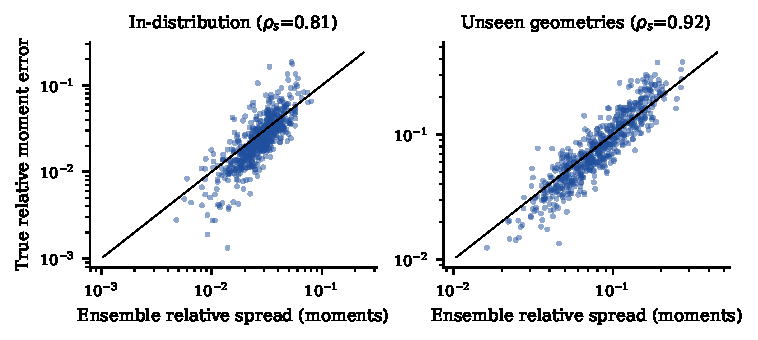
\includegraphics[width=\textwidth]{fig_uq_scatter.pdf}
\caption{Frame-level ensemble spread of the end moments $s$ (Eq.~\ref{eq:score}) against the true relative moment error for the four test sets. Black line: $e_M=s$; red dashed line: split-conformal bound $\hat a s$ calibrated on the validation frames.}\label{fig:uqscatter}
\end{figure}

The ensemble spread ranks the frames by their actual error well on in-distribution frames, on unseen geometries and on the design-driven frames (Spearman $\rho_s=0.81$, $0.92$ and $0.75$; Table~\ref{tab:uq} and Fig.~\ref{fig:uqscatter}), and the $\pm2\sigma$ intervals of the end moments contain 92\%, 92\% and 94\% of the PyNite values, close to the nominal 95\%. It is much weaker for unseen load patterns ($\rho_s=0.66$, coverage 67\%): the networks agree with each other on these frames while being wrong together, the known failure mode of ensembles under distribution shift~\cite{ovadia2019shift}. The label-free equilibrium residual of the raw prediction is a weaker indicator ($\rho_s=0.43$--$0.74$), which is why it is not used for referral.

\begin{table}[t]
\centering
\caption{Stage 1 of the referral rule: fraction of frames (\%) flagged as outside the training domain by the Mahalanobis distance of the frame descriptors, threshold at the 99th percentile of the validation frames.}\label{tab:ooddomain}
\footnotesize
\begin{tabular}{lrrrrr}
\toprule
Descriptors & Validation & ID & OOD-G & OOD-L & DES \\
\midrule
\inputtable{tables/tab_ood_domain.tex}
\bottomrule
\end{tabular}
\end{table}

The domain check (Table~\ref{tab:ooddomain}) flags 1.7\% of the ID test frames, close to the 1\% calibrated on the validation frames, and 79\% of the OOD-G and 75\% of the OOD-L frames. The two descriptor groups detect different shifts: the geometry descriptors flag 68\% of the unseen geometries but only 1.5\% of the unseen load patterns, and the load-pattern descriptors flag 67\% of the unseen load patterns but only 9\% of the unseen geometries. The load-pattern check therefore supplies exactly the information that the ensemble spread lacks. All 149 OOD-L frames that pass the check are frames whose random bay pattern happened to leave every bay fully loaded, so that only the lateral profile is new; the 129 OOD-G frames that pass are one step beyond the training range (45 have six storeys, 68 have five bays and at most five storeys). The check also flags 20\% of the design-driven frames, mainly because of their high gravity-to-lateral load ratio, their small roof share of the lateral load and their stiff material ($E$ at the upper end of the range), although the surrogate is accurate on all of them. The domain check is therefore conservative, which costs FE analyses but not accuracy.

\begin{table}[t]
\centering
\caption{Two-stage referral rule with thresholds fixed on the validation frames ($\hat a=1.41$ for $\alpha=0.1$). Referred: by the domain check, by the conformal bound $\hat a s>\tau$ and in total (\%). Coverage: share of in-domain frames with $e_M\le\hat a s$. Violation: share of accepted frames with $e_M>\tau$. p95: 95th percentile of $e_M$ over the accepted frames and over all frames (\%).}\label{tab:oodpolicy}
\footnotesize
\begin{adjustbox}{max width=\textwidth}
\begin{tabular}{llrrrrrrr}
\toprule
$\tau$ & Set & Domain & Bound & Total & Coverage & Violation & p95 accepted & p95 all \\
\midrule
\inputtable{tables/tab_ood_policy.tex}
\bottomrule
\end{tabular}
\end{adjustbox}
\end{table}

Table~\ref{tab:oodpolicy} evaluates the complete rule, whose two thresholds were fixed on the validation frames before the test sets were used. With a tolerance of $\tau=10\%$ on the relative moment error, the rule refers 2.2\% of the ID frames and accepts the rest with a violation rate of 1.4\% (frames whose true error exceeds 10\% although accepted). On unseen geometries it refers 86\% of the frames and the accepted 14\% have a 95th-percentile error of 7.7\% and a violation rate of 1.2\%, compared with a 95th percentile of 22.6\% and 35\% of frames above 10\% without referral. On unseen load patterns it refers 75\% and the accepted frames have a violation rate of 1.4\%. On the design-driven frames 20\% are referred by the domain check and none of the accepted frames exceeds 10\% (largest accepted error 4.8\%). With $\tau=5\%$ the violation rates are 3.5\% (ID), 17\% (OOD-G, 12 accepted frames), 5.4\% (OOD-L) and 0\% (DES), at the cost of referring 28\% of the ID frames. The conformal bound covers the true error in 90\% (ID), 94\% (OOD-G) and 99\% (DES) of the in-domain frames, matching the nominal 90\%, but only in 84\% of the in-domain OOD-L frames, so the coverage guarantee, which assumes exchangeability with the calibration frames, holds only approximately once the load pattern changes; the domain check is what keeps the accepted OOD-L frames safe. These numbers are the honest cost of the safety: the rule cannot make the surrogate accurate where it is not, but it makes the referral decision before the FE result is known and with thresholds that were not tuned on the test data.

\begin{figure}[p]
\centering
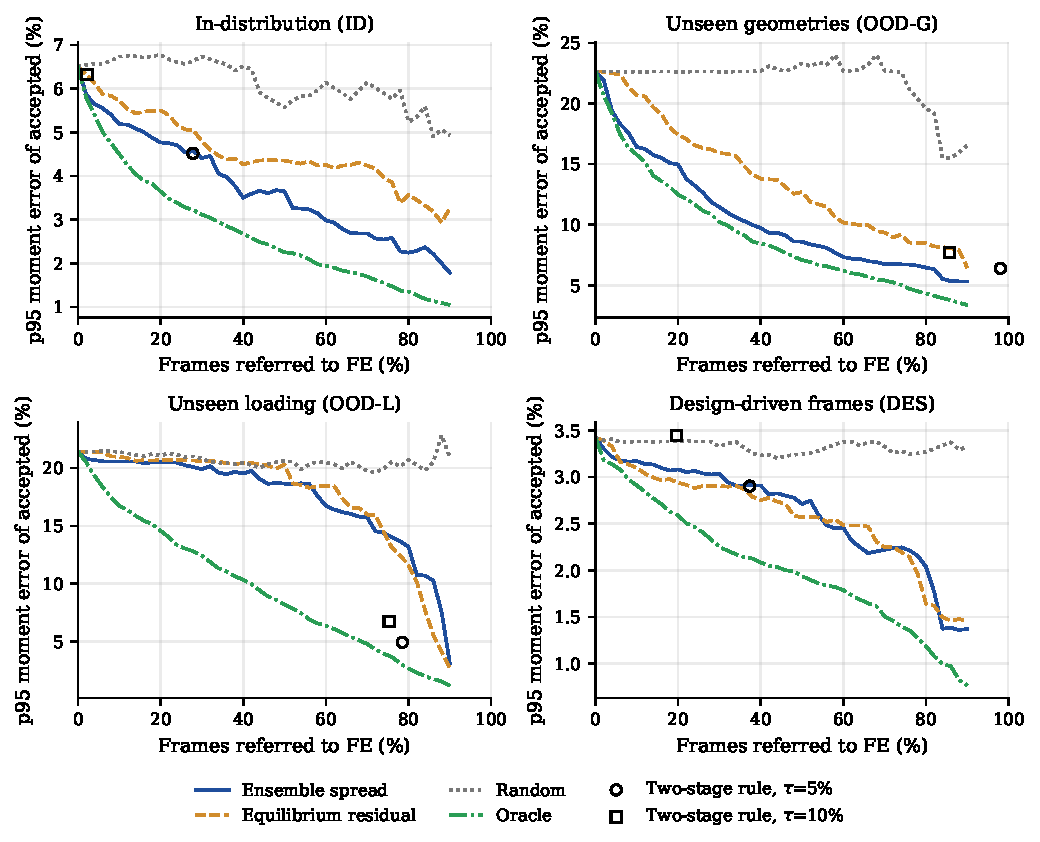
\includegraphics[width=\textwidth]{fig_triage.pdf}
\caption{Risk--coverage curves: 95th percentile of the moment error over the accepted predictions when the frames with the largest scores are referred to PyNite, for the ensemble spread, the equilibrium residual, random referral and an oracle ranking by the true error. Markers: operating points of the two-stage rule with validation-calibrated thresholds (Table~\ref{tab:oodpolicy}). The curves are computed on the test sets and serve only to describe the ranking quality.}\label{fig:triage}
\end{figure}

Figure~\ref{fig:triage} complements the rule with risk--coverage curves. On the ID set, referring the 20\% of frames with the largest spread lowers the 95th-percentile moment error from 6.5\% to 4.8\% and catches 78\% of the 1.5\% of frames with errors above 10\%. On unseen geometries it lowers the tail from 22.6\% to 15.0\%; on unseen load patterns the spread-based ranking is little better than random (21.4\%$\to$20.5\%), which is why the domain check is needed.


\subsection{Adaptive FE data generation}\label{sec:adaptive}
The adaptive study starts from 200 randomly chosen PyNite analyses and adds 200 per round up to 1{,}200, training a three-network ensemble (100 epochs) in every round; the whole study is repeated with two random seeds, and Fig.~\ref{fig:adaptive} shows the seed mean with the range of the two runs. Table~\ref{tab:adaptive} lists the errors at the final budget. Because these ensembles are smaller and trained on fewer frames for fewer epochs, their errors are higher than those of the main model in Table~\ref{tab:main}.

\begin{figure}[t]
\centering
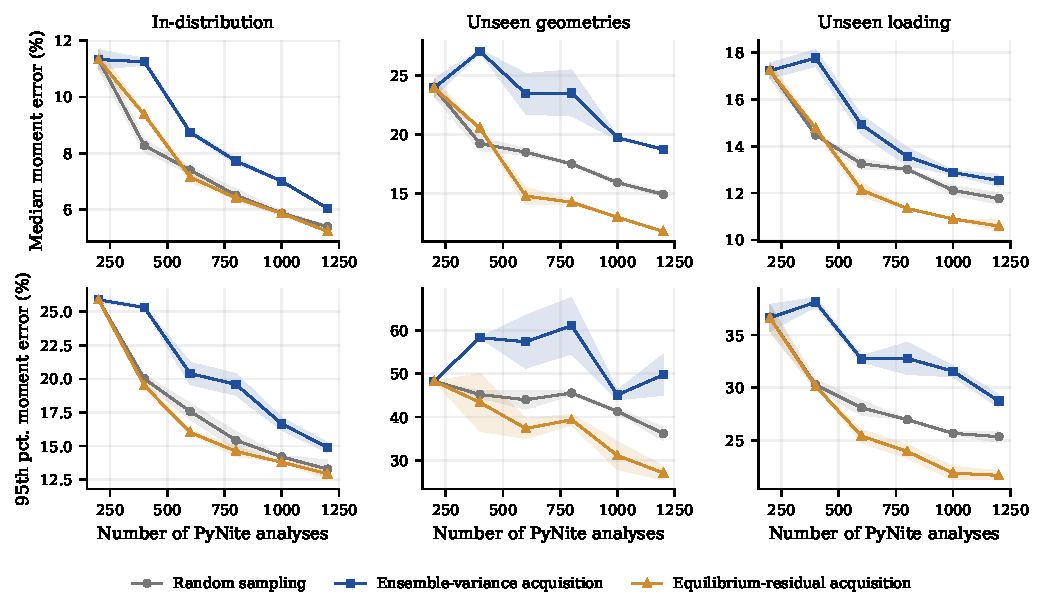
\includegraphics[width=\textwidth]{fig_adaptive.pdf}
\caption{Moment error (median, top; 95th percentile, bottom) versus the number of PyNite analyses used for training, for three acquisition rules. Lines: mean of two seeds; bands: range of the two seeds. Predictions include the variance-weighted projection.}\label{fig:adaptive}
\end{figure}

\begin{table}[t]
\centering
\caption{Errors (\%) after 1{,}200 PyNite analyses for each acquisition rule (mean of two seeds): median and 95th percentile of the moment error and median horizontal displacement error.}\label{tab:adaptive}
\scriptsize
\setlength{\tabcolsep}{3.5pt}
\begin{adjustbox}{max width=\textwidth}
\begin{tabular}{lrrrrrrrrr}
\toprule
& \multicolumn{3}{c}{In-distribution} & \multicolumn{3}{c}{Unseen geometries} & \multicolumn{3}{c}{Unseen loading}\\
\cmidrule(lr){2-4}\cmidrule(lr){5-7}\cmidrule(lr){8-10}
Acquisition & $e_M$ & $e_M$ (p95) & $e_{u_x}$ & $e_M$ & $e_M$ (p95) & $e_{u_x}$ & $e_M$ & $e_M$ (p95) & $e_{u_x}$\\
\midrule
\inputtable{tables/tab_adaptive.tex}
\bottomrule
\end{tabular}
\end{adjustbox}
\end{table}

Two findings stand out. First, selecting the frames with the largest ensemble variance is \emph{worse} than random sampling on all three test sets and for both seeds (median moment error 6.0\% vs.\ 5.4\% ID, 18.8\% vs.\ 14.9\% OOD-G at 1{,}200 analyses). Greedy top-$B$ selection by variance concentrates the budget on the most extreme corners of the design space, typically frames with very flexible members or unusual stiffness ratios, at the expense of coverage of the bulk of the distribution; a batch of 200 such frames is also highly redundant. Second, selecting the frames whose raw prediction is furthest from equilibrium is the best of the three rules for the member forces on every test set: at 1{,}200 analyses the median moment error is 5.2\% (random 5.4\%) on ID frames, 11.8\% (14.9\%) on unseen geometries and 10.6\% (11.8\%) on unseen loading, and the 95th percentile on unseen geometries falls from 36.2\% to 27.1\%. On unseen geometries the equilibrium-residual rule reaches the final error of random sampling after 600 analyses, i.e.\ with half the FE budget, and on unseen loading after 800. The gain is specific to forces: the displacement errors are similar to or slightly larger than with random sampling (Table~\ref{tab:adaptive}), which is expected, since the residual measures the admissibility of the forces only. With two seeds, the differences between the equilibrium-residual rule and random sampling on the ID set are within the seed-to-seed spread, whereas those on the unseen sets are consistent across both seeds.


\subsection{Computational cost}\label{sec:cost}
Timings were measured serially on the otherwise idle machine (Section~\ref{sec:protocol}), five times for 200 frames of each test set (Table~\ref{tab:timing}). Besides PyNite, two other solvers were timed on the same frames for both load cases: OpenSeesPy and the vectorised sparse direct-stiffness solver written for the verification (Section~\ref{sec:validation}), which represents an optimised minimal FE pipeline for this problem class. A PyNite analysis of one frame (two load cases, including model construction and result extraction) costs $33.6\pm1.6$\,ms for ID frames and $98.0\pm4.0$\,ms for the larger OOD-G frames. Evaluated in batches, the proposed surrogate costs 2.7\,ms (ID and OOD-L) and 7.0\,ms (OOD-G) per frame, including the Python feature construction (the largest part), the five-network ensemble and the projection (0.1--0.6\,ms), i.e.\ 12--14 times less than PyNite. For a single frame evaluated in isolation the overhead of the network framework dominates and the surrogate (20--87\,ms) is not faster than PyNite.

\begin{table}[t]
\centering
\caption{Wall-clock time per frame (ms; mean $\pm$ standard deviation over five repetitions of 200 frames, 4-core 2.1\,GHz CPU, networks evaluated with 4 threads): PyNite, OpenSeesPy and the sparse direct-stiffness solver (DSM) for both load cases; the proposed surrogate evaluated in batches and for one frame alone; batched speed-up relative to PyNite and to the DSM solver.}\label{tab:timing}
\footnotesize
\setlength{\tabcolsep}{3pt}
\begin{adjustbox}{max width=\textwidth}
\begin{tabular}{lrrrrrrr}
\toprule
Set & PyNite & OpenSeesPy & DSM & Surrogate (batched) & Surrogate (single) & vs PyNite & vs DSM\\
\midrule
\inputtable{tables/tab_timing.tex}
\bottomrule
\end{tabular}
\end{adjustbox}
\end{table}

The comparison with an optimised solver changes the picture. OpenSeesPy and the sparse direct-stiffness solver analyse a frame in 1.2--2.8\,ms, faster than the batched surrogate on every test set (speed-up of the surrogate over the DSM solver 0.34--0.65). Most of the cost of a PyNite analysis is the construction of the general three-dimensional model and the extraction of results through its object interface, not the solution of the linear system, which for frames with at most a few hundred DOFs takes well under a millisecond. Against PyNite, the batched surrogate pays back its one-off cost (about 41\,min of CPU time to train the five networks, while the 3{,}000 training analyses cost about 2\,min) only after roughly $8\times10^4$ ID frames without referral and $1.1\times10^5$ with 20\% of the frames referred to PyNite; against an optimised solver it never does. For first-order linear analysis of frames of this size the surrogate therefore offers no speed advantage over a well-implemented FE solver. Its value in this setting lies elsewhere: a differentiable, batched map from the frame parameters to the full response with a calibrated referral rule, which is useful for gradient-based design and for screening, and a template for analyses that are genuinely expensive (nonlinear, dynamic, or much larger models), which this paper does not test.


%% ---------------------------------------------------------------------------
\section{Discussion}\label{sec:discussion}

\paragraph{Answer to the research question} Within the design space it was trained on, the surrogate predicts member forces accurately enough to replace most repeated linear analyses at the level of preliminary design and screening: the median error of the end-moment field is 2.4\%, the largest end moment of a frame is within 0.8\% at the median, and the forces are exactly in equilibrium with the loads. Displacements are less accurate (median 4.5\% for the horizontal displacement field, 4.9\% for the governing drift). Outside the training space the median errors roughly triple and the 95th percentile of the moment error exceeds 20\%; the surrogate is then usable only together with a mechanism that sends doubtful cases back to the FE solver. That mechanism works for unseen geometries, where the ensemble spread ranks the errors well, but not for unseen load patterns, where the ensemble is confidently wrong. The answer is therefore a qualified yes: the surrogate can reduce repeated FE analysis inside a validated domain and, with referral, for moderately larger frames, but it is not a substitute for FE analysis on load patterns that the training data did not cover.

\paragraph{What the constraints buy} The constraints that hold exactly by construction contribute in two different ways. Exact load-case superposition and dimensional scaling are an \emph{accuracy} device: they remove the need to learn the dependence on the load intensities and on $E$, and they make the lateral and gravity responses equally well conditioned, which roughly halves the displacement errors (Table~\ref{tab:ablation}). The equilibrium projection is primarily an \emph{admissibility} device: it guarantees that the forces are in equilibrium, which a soft penalty does not achieve, and with a variance-weighted metric it also improves the forces, strongly for the axial forces and modestly for the moments. With a poorly chosen metric the projection can degrade the moments, so the metric is an essential part of the method rather than a detail. The projection does not enforce compatibility or the constitutive law: the predicted displacements and forces are not guaranteed to be consistent with each other, and imposing both equilibrium and compatibility exactly would amount to solving the FE problem.

\paragraph{Uncertainty as a decision tool} The two uses of uncertainty behaved differently. At deployment, the ensemble spread is a good indicator of which frames to refer to FE analysis for in-distribution and geometrically extrapolated frames, but its calibration collapses under a change of load pattern (coverage of the $\pm2\sigma$ intervals 67\% instead of 92\%). During training-set construction, greedy acquisition by ensemble variance was worse than random sampling, whereas acquisition by the equilibrium residual, a physics-based indicator that requires no labels, was the best rule for the member forces and halved the FE budget needed to reach a given accuracy on unseen geometries. A plausible explanation is that the residual is driven by the parts of the response that statics can check, whereas the variance also rewards the most atypical parameter combinations, which contribute little to the bulk of the test distribution. Batch-diversity and density-weighted acquisition rules, which are common remedies, were not tested.

\paragraph{Cost} The per-frame speed-up of the batched surrogate over PyNite is about 10--15, and 3.3--3.8 with 20\% referral. Because a linear PyNite analysis of these frames takes only 30--100\,ms, the one-off training cost of the ensemble (about 41\,min of CPU time) is recovered only after tens of thousands of evaluations. This is an honest limitation of applying the method to cheap linear analyses and should be weighed against the specific use case; the accuracy, admissibility and uncertainty results do not depend on it.

\paragraph{Limitations} The study is restricted to planar, regular, multi-storey moment frames with prismatic members, rigid joints, uniformly distributed beam loads and floor-level lateral forces, analysed with first-order linear elasticity. Sections and loads were sampled independently, so many frames would not satisfy serviceability limits; the dimensionless formulation makes the relative errors invariant to this, but the parameter correlations of designed frames are not represented. All results come from one dataset, one training run of each main model and two seeds of the adaptive study, so small differences (for example between the two projection metrics on in-distribution frames) should not be over-interpreted. The adaptive study is retrospective: candidates were labelled in advance and their labels revealed only on request, which yields exact budget accounting but not the scheduling overheads of a live FE loop. Timings were measured on one CPU with Python implementations of both the surrogate and PyNite.

\paragraph{Outlook} Natural extensions are a mixed formulation that also enforces compatibility through the member flexibilities, extension to three-dimensional frames, braced systems and second-order (P-$\Delta$) analysis, in which the FE cost is higher and superposition no longer holds exactly, explicit domain checks on the load pattern to complement the ensemble, and diversity-aware batch acquisition.

%% ---------------------------------------------------------------------------
\section{Conclusions}\label{sec:conclusions}

A mechanics-constrained surrogate modelling framework for the linear response of planar moment frames was developed and evaluated on 7{,}200 PyNite analyses. A graph network ensemble predicts nodal displacements and member basic forces in a dimensionless, load-case-separated form, so that superposition, homogeneity in the loads and in Young's modulus and the boundary conditions hold exactly; an equilibrium projection with an uncertainty-weighted metric makes the predicted forces statically admissible; and the uncertainty estimate decides which frames are analysed with PyNite during training and at deployment. The main conclusions are:
\begin{enumerate}
\item On in-distribution frames the surrogate reaches median errors of 2.4\% for the end-moment field, 0.6\% for the axial forces, 0.8\% for the largest end moment and 4.5\% for the horizontal displacements, four to six times lower than the best of five regression and ML baselines given identical features.
\item On unseen geometries and unseen load patterns the median moment errors are 7.5\% and 8.7\% (best baseline 22.1--22.5\% and 16.8--17.3\%), but the 95th percentiles exceed 20\%.
\item The equilibrium projection reduces the out-of-balance force from 4--16\% (raw ensemble) and up to 120\% (baselines) to machine precision for every model; with a variance-weighted metric it also reduces the force errors, whereas a Euclidean metric can increase the moment errors. A soft equilibrium penalty is ineffective.
\item Exact load-case superposition roughly halves the displacement errors compared with a single load scale.
\item The ensemble spread ranks the frame errors well for in-distribution frames and unseen geometries (Spearman 0.81 and 0.92) and supports effective FE referral there, but it is poorly calibrated for unseen load patterns.
\item For adaptive data generation, acquisition by the equilibrium residual of the raw prediction gave the most accurate member forces and reached the accuracy of 1{,}200 random analyses on unseen geometries with 600 analyses, whereas acquisition by ensemble variance was worse than random sampling.
\item The batched surrogate is about 10--15 times faster than a PyNite analysis per frame, but the training cost is recovered only after tens of thousands of evaluations for analyses as cheap as those considered here.
\end{enumerate}
The framework is therefore best viewed as a reliability layer that makes learned structural surrogates statically admissible and self-aware of their limits, rather than as a replacement for FE analysis.


\section*{Data and code availability}
All scripts used to generate the PyNite dataset, train the models, run the experiments and produce every figure and table are in the \texttt{research/surrogate} folder of the PyNite fork (\url{https://github.com/karthice1/Pynite}). The dataset is regenerated deterministically from the seeds in \texttt{generate\_dataset.py}.

\section*{CRediT authorship contribution statement}
To be completed by the authors.

\section*{Declaration of competing interest}
The authors declare that they have no known competing financial interests or personal relationships that could have appeared to influence the work reported in this paper.

\section*{Declaration of generative AI and AI-assisted technologies in the manuscript preparation process}
During the preparation of this work the authors used an AI assistant (Claude, Anthropic) to write the analysis code, run the experiments and draft the manuscript. All numerical results were produced by the released scripts. After using this tool, the authors reviewed and edited the content as needed and take full responsibility for the content of the published article.

\bibliographystyle{elsarticle-num}
\bibliography{references}

\end{document}
